\documentclass{report}\usepackage[]{graphicx}\usepackage[]{color}
%% maxwidth is the original width if it is less than linewidth
%% otherwise use linewidth (to make sure the graphics do not exceed the margin)
\makeatletter
\def\maxwidth{ %
  \ifdim\Gin@nat@width>\linewidth
    \linewidth
  \else
    \Gin@nat@width
  \fi
}
\makeatother

\definecolor{fgcolor}{rgb}{0.345, 0.345, 0.345}
\newcommand{\hlnum}[1]{\textcolor[rgb]{0.686,0.059,0.569}{#1}}%
\newcommand{\hlstr}[1]{\textcolor[rgb]{0.192,0.494,0.8}{#1}}%
\newcommand{\hlcom}[1]{\textcolor[rgb]{0.678,0.584,0.686}{\textit{#1}}}%
\newcommand{\hlopt}[1]{\textcolor[rgb]{0,0,0}{#1}}%
\newcommand{\hlstd}[1]{\textcolor[rgb]{0.345,0.345,0.345}{#1}}%
\newcommand{\hlkwa}[1]{\textcolor[rgb]{0.161,0.373,0.58}{\textbf{#1}}}%
\newcommand{\hlkwb}[1]{\textcolor[rgb]{0.69,0.353,0.396}{#1}}%
\newcommand{\hlkwc}[1]{\textcolor[rgb]{0.333,0.667,0.333}{#1}}%
\newcommand{\hlkwd}[1]{\textcolor[rgb]{0.737,0.353,0.396}{\textbf{#1}}}%

\usepackage{framed}
\makeatletter
\newenvironment{kframe}{%
 \def\at@end@of@kframe{}%
 \ifinner\ifhmode%
  \def\at@end@of@kframe{\end{minipage}}%
  \begin{minipage}{\columnwidth}%
 \fi\fi%
 \def\FrameCommand##1{\hskip\@totalleftmargin \hskip-\fboxsep
 \colorbox{shadecolor}{##1}\hskip-\fboxsep
     % There is no \\@totalrightmargin, so:
     \hskip-\linewidth \hskip-\@totalleftmargin \hskip\columnwidth}%
 \MakeFramed {\advance\hsize-\width
   \@totalleftmargin\z@ \linewidth\hsize
   \@setminipage}}%
 {\par\unskip\endMakeFramed%
 \at@end@of@kframe}
\makeatother

\definecolor{shadecolor}{rgb}{.97, .97, .97}
\definecolor{messagecolor}{rgb}{0, 0, 0}
\definecolor{warningcolor}{rgb}{1, 0, 1}
\definecolor{errorcolor}{rgb}{1, 0, 0}
\newenvironment{knitrout}{}{} % an empty environment to be redefined in TeX

\usepackage{alltt}

\usepackage[margin=1in,bottom=.5in,includehead,includefoot]{geometry}
\usepackage{hyperref}
\usepackage{alltt}
\usepackage{fancyhdr}
\pagestyle{fancy}
\usepackage{minitoc}
\fancyhf{}

%comment these lines out to revert to default font
\usepackage{kpfonts}
\usepackage[T1]{fontenc}
\usepackage{inconsolata}
\IfFileExists{upquote.sty}{\usepackage{upquote}}{}
\begin{document}

%% CREATE A TITLE PAGE 
%% WRITE A PREFACE 
%JV: Will eventually need a longer introduction with some details about downloading R, R Studio, etc. Also clarify the relationship between what OI Biostat shows vs. this book (e.g., difference between figures)

\setcounter{tocdepth}{1}
\dominitoc
\tableofcontents

\newpage 
\setcounter{chapter}{-1}
\chapter{Preface}
\minitoc

This text is a companion to \textit{Introductory Statistics for the Life and Biomedical Sciences}; while the main text focuses on statistical concepts and ideas, this supplement provides details about how to use the statistical computing language \textsf{R}.

All the datasets used in the text can be accessed by downloading the OIBiostat package from \textsf{R}. Run the following command to download the package:

%% These commands aren't going to work until we have uploaded the package to CRAN. Just skip it for now and require below.
\begin{knitrout}
\definecolor{shadecolor}{rgb}{0.969, 0.969, 0.969}\color{fgcolor}\begin{kframe}
\begin{alltt}
\hlkwd{install.packages}\hlstd{(}\hlstr{"OIBioStat"}\hlstd{)}  \hlcom{## make sure to include the quotations}
\end{alltt}
\end{kframe}
\end{knitrout}

The above command only needs to be run once. Each time a dataset in the package is needed, run the following command: 

\begin{knitrout}
\definecolor{shadecolor}{rgb}{0.969, 0.969, 0.969}\color{fgcolor}\begin{kframe}
\begin{alltt}
\hlkwd{require}\hlstd{(OIBioStat)} \hlcom{## note the lack of quotations here}
\end{alltt}
\end{kframe}
\end{knitrout}

\newpage 
\chapter{Introduction to Basic Techniques}
\minitoc

\vspace{0.5cm} 

This chapter introduces basic commands for manipulating datasets, including how to calculate numerical summaries, create tables from data, and make graphical plots. 

\section{Case study: preventing peanut allergies}

The \texttt{LEAP} dataset contains the results of the "Learning Early About Peanut Allergy" (LEAP) study, an experiment conducted to assess whether early exposure to peanut products reduces the probability of peanut allergies developing. To access the documentation associated with the dataset, run the following command: 

\begin{knitrout}
\definecolor{shadecolor}{rgb}{0.969, 0.969, 0.969}\color{fgcolor}\begin{kframe}
\begin{alltt}
\hlkwd{help}\hlstd{(LEAP)}
\end{alltt}
\end{kframe}
\end{knitrout}

A file will appear in the Help pane that provides some basic information about the dataset:

\begin{itemize}
\item \textbf{Description:} A general overview of the dataset. 
\item \textbf{Usage:} Instructions for how to load the dataset. 
\item \textbf{Format:} The names and descriptions of each variable in the dataset, including information about variable type and measurement units.
\item \textbf{Details:} Additional details about the conditions under which the data were collected.
\item \textbf{Source}: Information about where the data originates from.
\end{itemize}

To view the dataset itself, run:

\begin{knitrout}
\definecolor{shadecolor}{rgb}{0.969, 0.969, 0.969}\color{fgcolor}\begin{kframe}
\begin{alltt}
\hlkwd{View}\hlstd{(LEAP)}
\end{alltt}
\end{kframe}
\end{knitrout}

In the main console pane, a window will appear that shows the entire dataset. The variable names are displayed across the top, as the names of the columns. Data for each case in the study are contained within the rows. Note that the farthest left column shows the \textbf{indices}, which are computer-generated values that allow specific rows in the dataset to be accessed. These can be used to view a specific portion of the data.

For example, to print out data contained in the first 5 rows and first 3 columns of the data, use the following syntax:

\begin{knitrout}
\definecolor{shadecolor}{rgb}{0.969, 0.969, 0.969}\color{fgcolor}\begin{kframe}
\begin{alltt}
\hlstd{LEAP[}\hlnum{1}\hlopt{:}\hlnum{5}\hlstd{,}\hlnum{1}\hlopt{:}\hlnum{3}\hlstd{]}
\end{alltt}
\begin{verbatim}
##   participant.ID    treatment.group age.months
## 1    LEAP_100522 Peanut Consumption     6.0780
## 2    LEAP_103358 Peanut Consumption     7.5893
## 3    LEAP_105069   Peanut Avoidance     5.9795
## 4    LEAP_105328 Peanut Consumption     7.0308
## 5    LEAP_106377   Peanut Avoidance     6.4066
\end{verbatim}
\end{kframe}
\end{knitrout}

The bracket notation after the dataset name implies location; the syntax \texttt{dataset[rows,columns]} specifies rows 1 through 5 and columns 1 through 6. To access only the first 5 rows, but all the columns, leave an empty space where the columns would usually be specified:

\begin{knitrout}
\definecolor{shadecolor}{rgb}{0.969, 0.969, 0.969}\color{fgcolor}\begin{kframe}
\begin{alltt}
\hlcom{## note the space (or lack of text after the comma)}
\hlstd{LEAP[}\hlnum{1}\hlopt{:}\hlnum{5}\hlstd{, ]}
\end{alltt}
\begin{verbatim}
##   participant.ID    treatment.group age.months    sex primary.ethnicity
## 1    LEAP_100522 Peanut Consumption     6.0780 Female             Black
## 2    LEAP_103358 Peanut Consumption     7.5893 Female             White
## 3    LEAP_105069   Peanut Avoidance     5.9795   Male             White
## 4    LEAP_105328 Peanut Consumption     7.0308 Female             White
## 5    LEAP_106377   Peanut Avoidance     6.4066   Male             White
##   overall.V60.outcome
## 1            PASS OFC
## 2            PASS OFC
## 3            PASS OFC
## 4            PASS OFC
## 5            PASS OFC
\end{verbatim}
\end{kframe}
\end{knitrout}

Alternatively, since there are 6 columns in the dataset, the command \texttt{LEAP[1:5,1:6]} would also achieve the same result. This is a common theme in \textsf{R} -- there can be several ways to accomplish a desired result. 

\textit{OI Biostat} Table 1.1 shows the participant ID, treatment group, and overall outcome for five patients. It is not specified in the main text, but the data are specifically from rows 1, 2, 3, 529, and 530. The command \texttt{c()} can be used to bind the row numbers into a list, as well as to create a list of the desired columns. Columns can be referred to by name, instead of by number:

\begin{knitrout}
\definecolor{shadecolor}{rgb}{0.969, 0.969, 0.969}\color{fgcolor}\begin{kframe}
\begin{alltt}
\hlcom{## OI Biostat Table 1.1}
\hlstd{LEAP[}\hlkwd{c}\hlstd{(}\hlnum{1}\hlstd{,} \hlnum{2}\hlstd{,} \hlnum{3}\hlstd{,} \hlnum{529}\hlstd{,} \hlnum{530}\hlstd{),}\hlkwd{c}\hlstd{(}\hlstr{"participant.ID"}\hlstd{,} \hlstr{"treatment.group"}\hlstd{,}
                         \hlstr{"overall.V60.outcome"}\hlstd{)]}
\end{alltt}
\begin{verbatim}
##     participant.ID    treatment.group overall.V60.outcome
## 1      LEAP_100522 Peanut Consumption            PASS OFC
## 2      LEAP_103358 Peanut Consumption            PASS OFC
## 3      LEAP_105069   Peanut Avoidance            PASS OFC
## 639    LEAP_994047   Peanut Avoidance            PASS OFC
## 640    LEAP_997608 Peanut Consumption            PASS OFC
\end{verbatim}
\end{kframe}
\end{knitrout}

Two-way summary tables organize the data according to two variables and display the number of counts matching each combination of variable categories. The following code corresponds to \textit{OI~Biostat} Table~1.2, which groups participants into categories based on treatment group and overall outcome. In the \texttt{table()} command, the first variable specifies the rows and the second variable specifies the columns. The addition of the \texttt{addmargins()} command prints the sums of the rows and columns on the sides of the table.

\begin{knitrout}
\definecolor{shadecolor}{rgb}{0.969, 0.969, 0.969}\color{fgcolor}\begin{kframe}
\begin{alltt}
\hlcom{## Table 1.2}
\hlkwd{table}\hlstd{(LEAP}\hlopt{$}\hlstd{treatment.group, LEAP}\hlopt{$}\hlstd{overall.V60.outcome)}
\end{alltt}
\begin{verbatim}
##                     
##                      FAIL OFC PASS OFC
##   Peanut Avoidance         36      227
##   Peanut Consumption        5      262
\end{verbatim}
\begin{alltt}
\hlkwd{addmargins}\hlstd{(}\hlkwd{table}\hlstd{(LEAP}\hlopt{$}\hlstd{treatment.group, LEAP}\hlopt{$}\hlstd{overall.V60.outcome))}
\end{alltt}
\begin{verbatim}
##                     
##                      FAIL OFC PASS OFC Sum
##   Peanut Avoidance         36      227 263
##   Peanut Consumption        5      262 267
##   Sum                      41      489 530
\end{verbatim}
\end{kframe}
\end{knitrout}


\section{Data Basics}

Entire datasets can be partitioned into data frames using bracket notation. For example, \textit{OI Biostat} Table 1.3 shows a data frame consisting of rows 1-3 and 150 (and all columns) from the \texttt{frog.altitude} dataset. The data frame can then be given a specific name, such as \texttt{frog.df}, and directly called on for later operations.

%%JV: order of variables should be the same between companion and oi biostat

\begin{knitrout}
\definecolor{shadecolor}{rgb}{0.969, 0.969, 0.969}\color{fgcolor}\begin{kframe}
\begin{alltt}
\hlcom{## Table 1.3}
\hlstd{frog.df} \hlkwb{=} \hlstd{frog.altitude.data[}\hlkwd{c}\hlstd{(}\hlnum{1}\hlopt{:}\hlnum{3}\hlstd{,} \hlnum{150}\hlstd{),]}
\hlstd{frog.df}
\end{alltt}
\begin{verbatim}
##     altitude latitude clutch.size body.size clutch.volume egg.size
## 1   3,462.00    34.82    181.9701  3.630781      177.8279 1.949845
## 2   3,462.00    34.82    269.1535  3.630781      257.0396 1.949845
## 3   3,462.00    34.82    158.4893  3.715352      151.3561 1.949845
## 150 2,597.00    34.05    537.0318        NA      776.2471 2.238721
\end{verbatim}
\end{kframe}
\end{knitrout}

Similarly, matrix notation can be used to create \textit{OI Biostat} Table 1.5.

\begin{knitrout}
\definecolor{shadecolor}{rgb}{0.969, 0.969, 0.969}\color{fgcolor}\begin{kframe}
\begin{alltt}
\hlcom{## Table 1.5}
\hlstd{famuss[}\hlkwd{c}\hlstd{(}\hlnum{1}\hlstd{,}\hlnum{2}\hlstd{,}\hlnum{3}\hlstd{,}\hlnum{595}\hlstd{),}\hlkwd{c}\hlstd{(} \hlstr{"sex"}\hlstd{,} \hlstr{"age"}\hlstd{,} \hlstr{"race"}\hlstd{,} \hlstr{"height"}\hlstd{,} \hlstr{"weight"}\hlstd{,} \hlstr{"actn3.r577x"}\hlstd{,}
                       \hlstr{"ndrm.ch"}\hlstd{)]}
\end{alltt}
\begin{verbatim}
##         sex age      race height weight actn3.r577x ndrm.ch
## 1    Female  27 Caucasian   65.0    199          CC    40.0
## 2      Male  36 Caucasian   71.7    189          CT    25.0
## 3    Female  24 Caucasian   65.0    134          CT    40.0
## 1348 Female  30 Caucasian   64.0    134          CC    43.8
\end{verbatim}
\end{kframe}
\end{knitrout}

\stepcounter{subsection}
\section{Numerical Data}

Numerical summaries can be quickly and easily calculated using \textsf{R}. The \texttt{summary()} command is one way to access several numerical summaries at once, including the minimum and maximum values of a variable:
\begin{knitrout}
\definecolor{shadecolor}{rgb}{0.969, 0.969, 0.969}\color{fgcolor}\begin{kframe}
\begin{alltt}
\hlkwd{summary}\hlstd{(frog.altitude.data}\hlopt{$}\hlstd{clutch.volume)}
\end{alltt}
\begin{verbatim}
##    Min. 1st Qu.  Median    Mean 3rd Qu.    Max. 
##   151.4   609.6   831.8   882.5  1096.0  2630.0
\end{verbatim}
\end{kframe}
\end{knitrout}

\subsection{Measures of center: mean and median}

The \textbf{mean} of a numerical value is the sum of all observations divided by the number of observations, where $x_1, x_2, \dots, x_n$ represent the $n$ observed values:

\begin{align*}
		\overline{x} = \frac{x_1+x_2+\cdots+x_n}{n}
\end{align*}

This calculation can be completed in \textsf{R} the same way as a hand calculation is done:
\begin{knitrout}
\definecolor{shadecolor}{rgb}{0.969, 0.969, 0.969}\color{fgcolor}\begin{kframe}
\begin{alltt}
\hlcom{# identify n, the number of observations in the data}
\hlstd{n} \hlkwb{=} \hlkwd{length}\hlstd{(frog.altitude.data}\hlopt{$}\hlstd{clutch.volume)}
\hlstd{n}
\end{alltt}
\begin{verbatim}
## [1] 431
\end{verbatim}
\begin{alltt}
\hlcom{# calculate the sum of all observations and divide by n}
\hlkwd{sum}\hlstd{(frog.altitude.data}\hlopt{$}\hlstd{clutch.volume)}\hlopt{/}\hlstd{n}
\end{alltt}
\begin{verbatim}
## [1] 882.474
\end{verbatim}
\end{kframe}
\end{knitrout}

Alternatively, the \textsf{R} function \texttt{mean()} can be directly applied to the variable of interest:
\begin{knitrout}
\definecolor{shadecolor}{rgb}{0.969, 0.969, 0.969}\color{fgcolor}\begin{kframe}
\begin{alltt}
\hlstd{x.bar} \hlkwb{=} \hlkwd{mean}\hlstd{(frog.altitude.data}\hlopt{$}\hlstd{clutch.volume)}
\hlstd{x.bar}
\end{alltt}
\begin{verbatim}
## [1] 882.474
\end{verbatim}
\begin{alltt}
\hlcom{## round to the first decimal}
\hlkwd{round}\hlstd{(x.bar,} \hlnum{1}\hlstd{)}
\end{alltt}
\begin{verbatim}
## [1] 882.5
\end{verbatim}
\end{kframe}
\end{knitrout}

To identify the \textbf{median} value, use the following command:

\begin{knitrout}
\definecolor{shadecolor}{rgb}{0.969, 0.969, 0.969}\color{fgcolor}\begin{kframe}
\begin{alltt}
\hlkwd{median}\hlstd{(frog.altitude.data}\hlopt{$}\hlstd{clutch.volume)}
\end{alltt}
\begin{verbatim}
## [1] 831.7638
\end{verbatim}
\end{kframe}
\end{knitrout}

\subsection{Measures of spread: standard deviation and variance}

The distance of a single observation from the mean is its \textbf{deviation}. The following command produces the deviations for the $1^{st}$, $2^{nd}$, $3^{rd}$, and $431^{th}$ observations in the \texttt{clutch.volume} variable.

\begin{knitrout}
\definecolor{shadecolor}{rgb}{0.969, 0.969, 0.969}\color{fgcolor}\begin{kframe}
\begin{alltt}
\hlstd{frog.altitude.data}\hlopt{$}\hlstd{clutch.volume[}\hlkwd{c}\hlstd{(}\hlnum{1}\hlstd{,}\hlnum{2}\hlstd{,}\hlnum{3}\hlstd{,}\hlnum{431}\hlstd{)]}\hlopt{-}\hlstd{x.bar}
\end{alltt}
\begin{verbatim}
## [1] -704.64604 -625.43440 -731.11786   50.78032
\end{verbatim}
\end{kframe}
\end{knitrout}

The sample \textbf{standard deviation} is computed as the square root of the \textbf{variance}, which is the sum of squared deviations divided by the number of observations minus 1. 

\begin{align*}
		s = \sqrt{\frac{({x_1 - \overline{x})}^{2}+({x_2 - \overline{x})}^{2}+\cdots+({x_n - \overline{x})}^{2}}{n-1}}
\end{align*}

The following steps illustrate how to calculate the variance and standard deviation using the formula: 

\begin{knitrout}
\definecolor{shadecolor}{rgb}{0.969, 0.969, 0.969}\color{fgcolor}\begin{kframe}
\begin{alltt}
\hlcom{# calculate all deviations}
\hlstd{dev} \hlkwb{=} \hlstd{frog.altitude.data}\hlopt{$}\hlstd{clutch.volume} \hlopt{-} \hlstd{x.bar}

\hlcom{# sum the squares of the deviations and divide by n - 1}
\hlstd{var} \hlkwb{=} \hlstd{(}\hlkwd{sum}\hlstd{(dev}\hlopt{^}\hlnum{2}\hlstd{))}\hlopt{/}\hlstd{(n}\hlopt{-}\hlnum{1}\hlstd{)}
\hlstd{var}
\end{alltt}
\begin{verbatim}
## [1] 143680.9
\end{verbatim}
\begin{alltt}
\hlcom{# take the square root of the variance}
\hlstd{sd} \hlkwb{=} \hlkwd{sqrt}\hlstd{(var)}
\hlstd{sd}
\end{alltt}
\begin{verbatim}
## [1] 379.0527
\end{verbatim}
\end{kframe}
\end{knitrout}

Alternatively, use the \textsf{R} functions \texttt{var()} and \texttt{sd()}:

\begin{knitrout}
\definecolor{shadecolor}{rgb}{0.969, 0.969, 0.969}\color{fgcolor}\begin{kframe}
\begin{alltt}
\hlkwd{var}\hlstd{(frog.altitude.data}\hlopt{$}\hlstd{clutch.volume)}
\end{alltt}
\begin{verbatim}
## [1] 143680.9
\end{verbatim}
\begin{alltt}
\hlkwd{sd}\hlstd{(frog.altitude.data}\hlopt{$}\hlstd{clutch.volume)}
\end{alltt}
\begin{verbatim}
## [1] 379.0527
\end{verbatim}
\end{kframe}
\end{knitrout}


%To calculate the variance, you can follow a few steps:
%\begin{enumerate}
%\item Obtain the deviation of each data point from the mean, i.e. $x_i - \bar{x}$
%\item Square each of these deviations, i.e. $(x_i - \bar{x})^2$
%\item Sum all of the squares, i.e. $\sum_{i=1}^n (x_i - \bar{x})^2$
%\item To obtain the final value for variance, divide this sum by the number of observations minus 1, $n-1$, i.e. $(\frac{1}{n-1})\sum_{i=1}^n (x_i - \bar{x})^2$
%\item To obtain the standard deviation, take the square root of the variance, i.e $\sqrt{(\frac{1}{n-1})\sum_{i=1}^n (x_i - \bar{x})^2}$
%\end{enumerate}
%We go through these steps by hand here and compare to the $R$ function's output.

%<<>>=
%## Looking at a few sample values from text
%frog.altitude.data$clutch.volume[c(1,2,3,431)]-x.bar

%## Calculating variance by hand
%# Step 1: calculating all deviations
%diffs = frog.altitude.data$clutch.volume-x.bar

%# Steps 2-4:
%variance = sum(diffs^2)/(n-1)
%variance

%## Comparing to the R function's value
%var(frog.altitude.data$clutch.volume)

%## Step 5: obtaining standard deviation
%stand.dev = sqrt(variance)
%stand.dev
%sd(frog.altitude.data$clutch.volume)        ## compare to R function value
%@

Variability can also be measured using the \textbf{interquartile range (IQR)}, which equals the third quartile (the $75^{th}$ percentile) minus the first quartile (the $25^{th}$ percentile). 

\begin{knitrout}
\definecolor{shadecolor}{rgb}{0.969, 0.969, 0.969}\color{fgcolor}\begin{kframe}
\begin{alltt}
\hlkwd{IQR}\hlstd{(frog.altitude.data}\hlopt{$}\hlstd{clutch.volume)}
\end{alltt}
\begin{verbatim}
## [1] 486.9009
\end{verbatim}
\end{kframe}
\end{knitrout}

\subsection{Robust statistics}

In the \texttt{frog.altitude} dataset, there are four extreme values for clutch volume that are larger than 2,000 mm$^3$. To illustrate how the summary statistics are influenced by extreme values, \textit{OI Biostat} Table 1.15 shows summary statistics for the data without the four largest observations. 

The subset of the data with values less than 2,000 mm$^3$ can be pulled out by first specifying a logical condition, which assigns \texttt{TRUE} or \texttt{FALSE} to each entry. 

\begin{knitrout}
\definecolor{shadecolor}{rgb}{0.969, 0.969, 0.969}\color{fgcolor}\begin{kframe}
\begin{alltt}
\hlcom{# logical condition}
\hlstd{less.than.2000} \hlkwb{=} \hlstd{frog.altitude.data}\hlopt{$}\hlstd{clutch.volume}\hlopt{<=} \hlnum{2000}

\hlcom{# view the first 5 values}
\hlstd{less.than.2000[}\hlnum{1}\hlopt{:}\hlnum{5}\hlstd{]}
\end{alltt}
\begin{verbatim}
## [1] TRUE TRUE TRUE TRUE TRUE
\end{verbatim}
\end{kframe}
\end{knitrout}

Bracket notation can then be used to calculate summary statistics specifically for the values in \texttt{clutch.volume} that satisfy the logical condition.

\begin{knitrout}
\definecolor{shadecolor}{rgb}{0.969, 0.969, 0.969}\color{fgcolor}\begin{kframe}
\begin{alltt}
\hlcom{## robust estimates}
\hlkwd{median}\hlstd{(frog.altitude.data}\hlopt{$}\hlstd{clutch.volume[less.than.2000])}
\end{alltt}
\begin{verbatim}
## [1] 831.7638
\end{verbatim}
\begin{alltt}
\hlkwd{IQR}\hlstd{(frog.altitude.data}\hlopt{$}\hlstd{clutch.volume[less.than.2000])}
\end{alltt}
\begin{verbatim}
## [1] 493.9186
\end{verbatim}
\begin{alltt}
\hlcom{## non-robust estimates}
\hlkwd{mean}\hlstd{(frog.altitude.data}\hlopt{$}\hlstd{clutch.volume[less.than.2000])}
\end{alltt}
\begin{verbatim}
## [1] 867.9425
\end{verbatim}
\begin{alltt}
\hlkwd{sd}\hlstd{(frog.altitude.data}\hlopt{$}\hlstd{clutch.volume[less.than.2000])}
\end{alltt}
\begin{verbatim}
## [1] 349.1596
\end{verbatim}
\end{kframe}
\end{knitrout}

\subsection{Visualizing distributions of data}
While most numerical summaries can be calculated by hand, \textsf{R} is essential for creating graphical summaries.

\subsubsection{Histograms}
A \textbf{histogram} provides a view of data density. Observations are sorted into different bins based on their value, and the histogram shows the number of observations in each bin. The following command produces a histogram of the \texttt{clutch.volume} variable.

\begin{knitrout}
\definecolor{shadecolor}{rgb}{0.969, 0.969, 0.969}\color{fgcolor}\begin{kframe}
\begin{alltt}
\hlkwd{hist}\hlstd{(frog.altitude.data}\hlopt{$}\hlstd{clutch.volume)}
\end{alltt}
\end{kframe}
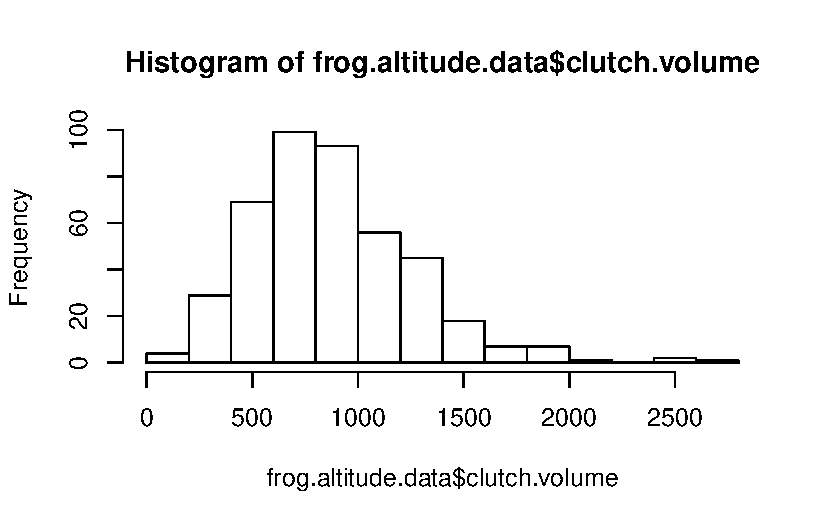
\includegraphics[width=\maxwidth]{figure/unnamed-chunk-19-1} 

\end{knitrout}

The \texttt{hist()} function takes several arguments:
\begin{itemize}
\item \texttt{x}: variable of interest
\item \texttt{breaks}: number of bins
\item \texttt{col}: color of the bars, enclosed in \texttt{""}
\item \texttt{xlab}: $x$-axis label, enclosed in \texttt{""}
\item \texttt{ylab}: $y$-axis label, enclosed in \texttt{""}
\item \texttt{xlim}: range of values for the $x$-axis, in the form \texttt{c(lower bound, upper bound)}
\item \texttt{ylim}: range of values for the $y$-axis, in the form \texttt{c(lower bound, upper bound)}
\item \texttt{main}: main title of the plot, enclosed in \texttt{""} 
\item \texttt{plot}: if \texttt{TRUE} (default), a histogram is plotted; otherwise, data about the histogram is returned
\end{itemize}

As seen above, not all arguments must be specified; only the \texttt{x} argument is necessary. When options are not specified, \textsf{R} uses the default options, such as the default color of white for the histogram bars.

The following command reproduces \textit{OI Biostat} Table 1.16 and Figure 1.17.

\begin{knitrout}
\definecolor{shadecolor}{rgb}{0.969, 0.969, 0.969}\color{fgcolor}\begin{kframe}
\begin{alltt}
\hlcom{## Table 1.16}
\hlkwd{hist}\hlstd{(frog.altitude.data}\hlopt{$}\hlstd{clutch.volume,} \hlkwc{breaks} \hlstd{=} \hlnum{14}\hlstd{,} \hlkwc{plot} \hlstd{=} \hlnum{FALSE}\hlstd{)}\hlopt{$}\hlstd{counts}
\end{alltt}
\begin{verbatim}
##  [1]  4 29 69 99 93 56 45 18  7  7  1  0  2  1
\end{verbatim}
\begin{alltt}
\hlcom{## Figure 1.17}
\hlkwd{hist}\hlstd{(}\hlkwc{x} \hlstd{= frog.altitude.data}\hlopt{$}\hlstd{clutch.volume,} \hlkwc{breaks} \hlstd{=} \hlnum{14}\hlstd{,} \hlkwc{col} \hlstd{=} \hlstr{"dodgerblue"}\hlstd{,}
     \hlkwc{xlab} \hlstd{=} \hlstr{"Clutch Volume"}\hlstd{,} \hlkwc{ylab} \hlstd{=} \hlstr{"Frequency"}\hlstd{,} \hlkwc{ylim} \hlstd{=} \hlkwd{c}\hlstd{(}\hlnum{0}\hlstd{,} \hlnum{100}\hlstd{),}
     \hlkwc{main} \hlstd{=} \hlstr{"Histogram of Clutch Volume Frequencies"}\hlstd{)}
\end{alltt}
\end{kframe}
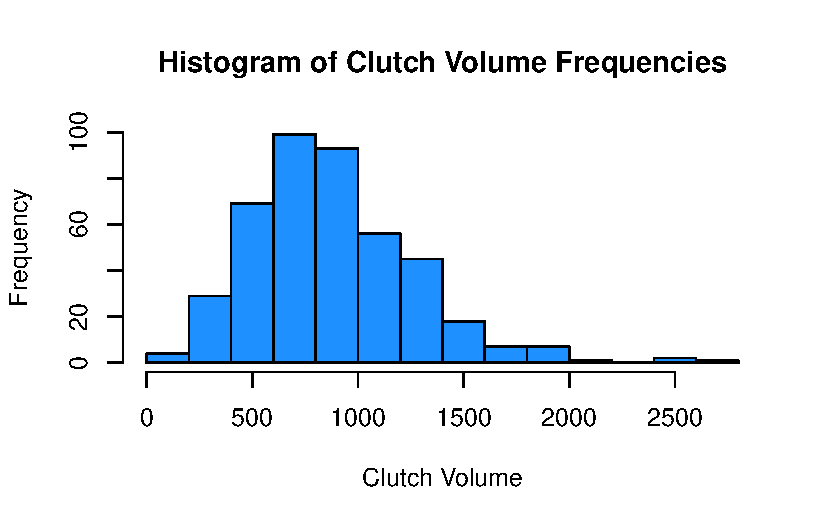
\includegraphics[width=\maxwidth]{figure/unnamed-chunk-20-1} 

\end{knitrout}


\subsubsection{Boxplots}

A \textbf{boxplot} uses five statistics to summarize a dataset, in addition to showing unusual observations. The following command produces a boxplot of the \texttt{clutch.volume} variable.

\begin{centering}
\begin{knitrout}
\definecolor{shadecolor}{rgb}{0.969, 0.969, 0.969}\color{fgcolor}\begin{kframe}
\begin{alltt}
\hlkwd{boxplot}\hlstd{(frog.altitude.data}\hlopt{$}\hlstd{clutch.volume)}
\end{alltt}
\end{kframe}
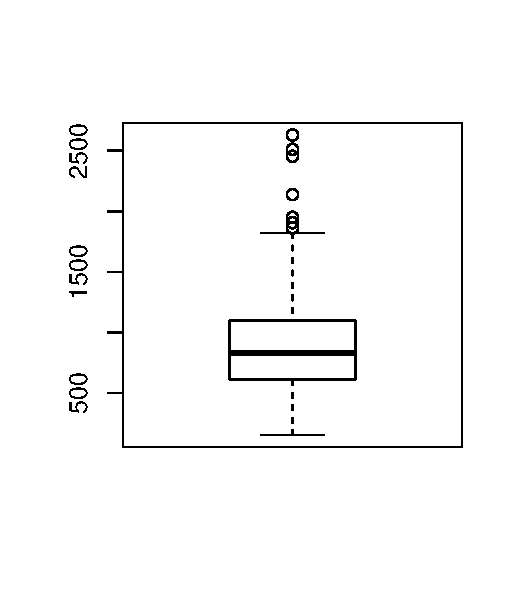
\includegraphics[width=\maxwidth]{figure/unnamed-chunk-21-1} 

\end{knitrout}
\end{centering}

Like the \texttt{hist()} function, the \texttt{boxplot()} function also takes several arguments that allow for certain parameters to be specified:
\begin{itemize}
\item \texttt{x}: variable of interest
\item \texttt{axes}: if \texttt{TRUE}, numbers are shown on the axes
\item \texttt{col}: color of the boxplot, enclosed in \texttt{""}
\item \texttt{xlab}: $x$-axis label, enclosed in \texttt{""}
\item \texttt{ylab}: $y$-axis label, enclosed in \texttt{""}
\item \texttt{xlim}: range of values for the $x$-axis, in the form \texttt{c(lower bound, upper bound)}
\item \texttt{ylim}: range of values for the $y$-axis, in the form \texttt{c(lower bound, upper bound)}
\item \texttt{main}: main title of the plot, enclosed in \texttt{""} 

\end{itemize}


%Another way to visualize data is with a boxplot.  The command for doing this in $R$ is \textit{boxplot()}, and it takes the following arguments:
%\begin{itemize}
%\item $x$: the variable you want to visualize
%\item $axes$: a TRUE/FALSE indicator that determines whether or not numbers are shown on the axes
%\item $col$: the color you want the fill inside your boxplot to be; if unspecified, it will be white; must be in quotation marks
%\item $xlab$: the label you would like the x-axis to have; must be in quotation marks
%\item $ylab$: the label you would like the y-axis to have; must be in quotation marks
%\item $xlim$: the range of values you would like the x-axis to have; of the form $c(lower bound, upper bound)$; fairly meaningless for a boxplot
%\item $ylim$: the range of values you would like the y-axis to have; of the form $c(lower bound, upper bound)$; be careful not to specify too much here because you can eliminate data of importance to the boxplot
%\item $main$: the title you would like the whole plot to have; must be in quotation marks
% \end{itemize}

The following command reproduces a simplified version of \textit{OI Biostat} Figure 1.19. 

\begin{centering}
\begin{knitrout}
\definecolor{shadecolor}{rgb}{0.969, 0.969, 0.969}\color{fgcolor}\begin{kframe}
\begin{alltt}
\hlcom{## Figure 1.19}
\hlkwd{boxplot}\hlstd{(}\hlkwc{x} \hlstd{= frog.altitude.data}\hlopt{$}\hlstd{clutch.volume,} \hlkwc{ylab} \hlstd{=} \hlstr{'Clutch Volume'}\hlstd{,} \hlkwc{axes} \hlstd{=} \hlnum{TRUE}\hlstd{,}
        \hlkwc{ylim} \hlstd{=} \hlkwd{range}\hlstd{(frog.altitude.data}\hlopt{$}\hlstd{clutch.volume))}
\end{alltt}
\end{kframe}
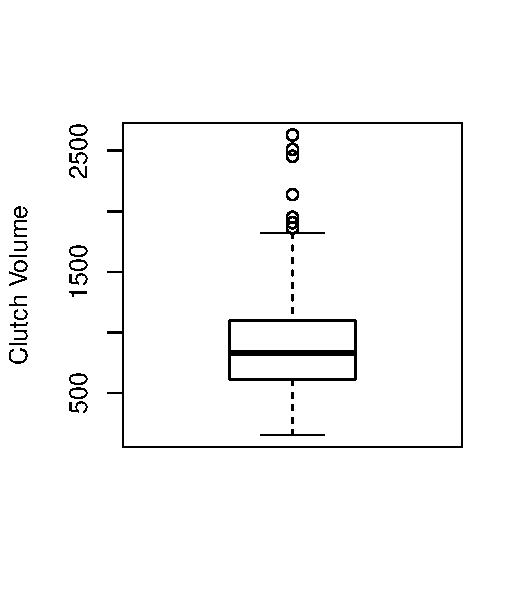
\includegraphics[width=\maxwidth]{figure/unnamed-chunk-22-1} 

\end{knitrout}
\end{centering}

\subsection{Scatterplots and correlation}
\textbf{Scatterplots} can be used to visualize the relationship between two numerical variables. In the \texttt{plot()} command, either a comma or a tilde can be used between the variable names; i.e., \texttt{plot(x,y)} versus \texttt{plot(y $\sim$ x)}.

\begin{knitrout}
\definecolor{shadecolor}{rgb}{0.969, 0.969, 0.969}\color{fgcolor}\begin{kframe}
\begin{alltt}
\hlkwd{plot}\hlstd{(frog.altitude.data}\hlopt{$}\hlstd{body.size, frog.altitude.data}\hlopt{$}\hlstd{clutch.volume)}
\end{alltt}
\end{kframe}

{\centering 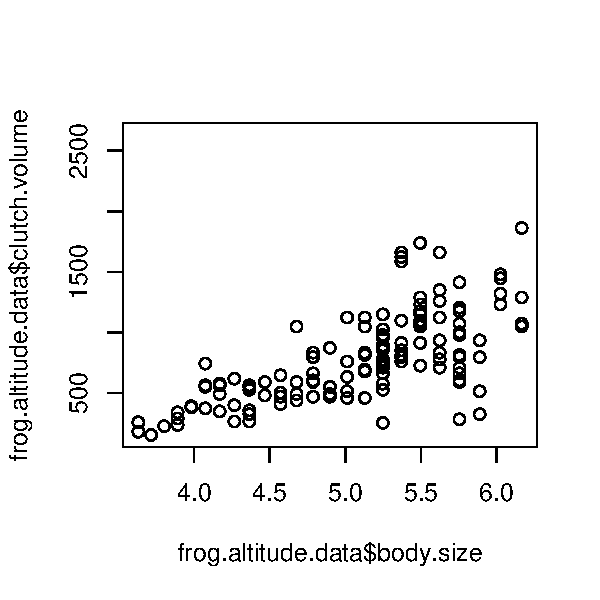
\includegraphics[width=\maxwidth]{figure/unnamed-chunk-23-1} 

}



\end{knitrout}

The \texttt{plot()} command takes the following arguments: 

\begin{itemize}
\item \texttt{x}: variable defining the $x$-coordinates 
\item \texttt{y}: variable defining the $y$-coordinates 
\item \texttt{col}: color of the dots, enclosed in \texttt{""}
\item \texttt{type}: by default, data points are marked with dots; other options include \texttt{"l"} which draws a line chart, or \texttt{"b"} which includes both dots and lines
\item \texttt{xlab}: $x$-axis label, enclosed in \texttt{""}
\item \texttt{ylab}: $y$-axis label, enclosed in \texttt{""}
\item \texttt{xlim}: range of values for the $x$-axis, in the form \texttt{c(lower bound, upper bound)}
\item \texttt{ylim}: range of values for the $y$-axis, in the form \texttt{c(lower bound, upper bound)}
\item \texttt{main}: main title of the plot, enclosed in \texttt{""} 
\end{itemize}

%The command for doing this is \textit{plot()}, and this function takes several arguments:
%\begin{itemize}
%\item $x$: the first variable you want to visualize; \textit{necessary to include}
%\item $y$: the second variable you may want to visualize; included if you want to consider two variables \textit{not necessary to include}
%\item $col$: the color you want your dots on the plot to be; if unspecified, they will be black; must be in quotation marks
%\item $type$: specifies how you want R to plot the data; if unspecified, you will end up with dots (in a scatterplot); other options include $"l"$ for lines between data points
%\item $xlab$: the label you would like the x-axis to have; must be in quotation marks
%\item $ylab$: the label you would like the y-axis to have; must be in quotation marks
%\item $xlim$: the range of values you would like the x-axis to have; of the form $c%(lower bound, upper bound)$
%\item $ylim$: the range of values you would like the y-axis to have; of the form $c(lower bound, upper bound)$
%\item $main$: the title you would like the whole plot to have; must be in quotation marks
%\end{itemize}

%The \textit{plot} command has an interesting feature that you can either specify your $x$ and $y$ variables by running $plot(x,y)$ or by running $plot(y~x)$.  Either command will give the same result.  Below provides an example of using the \textit{plot} command for one and two variables (corresponds to Figure 1.18 in the text):
%\begin{centering}
%<<fig.height=4, fig.width=4>>=
%# For one variable
%plot(frog.altitude.data$clutch.volume)
%@
%\end{centering}

The following command reproduces a simplified version of \textit{OI Biostat} Figure 1.20. The additional argument \texttt{pch} changes the appearance of the dots to filled dots, which is specified by \texttt{19}. 

\begin{centering}
\begin{knitrout}
\definecolor{shadecolor}{rgb}{0.969, 0.969, 0.969}\color{fgcolor}\begin{kframe}
\begin{alltt}
\hlcom{## Figure 1.20}
\hlkwd{plot}\hlstd{(frog.altitude.data}\hlopt{$}\hlstd{clutch.volume}\hlopt{~}\hlstd{frog.altitude.data}\hlopt{$}\hlstd{body.size,} \hlkwc{col} \hlstd{=} \hlstr{"dodgerblue"}\hlstd{,}
     \hlkwc{pch} \hlstd{=} \hlnum{19}\hlstd{,} \hlkwc{xlab} \hlstd{=} \hlstr{"Female Body Size (cm)"}\hlstd{,} \hlkwc{ylab} \hlstd{=} \hlkwd{expression}\hlstd{(}\hlstr{"Clutch Volume"} \hlopt{~} \hlstd{(mm}\hlopt{^}\hlnum{3}\hlstd{)))}
\end{alltt}
\end{kframe}
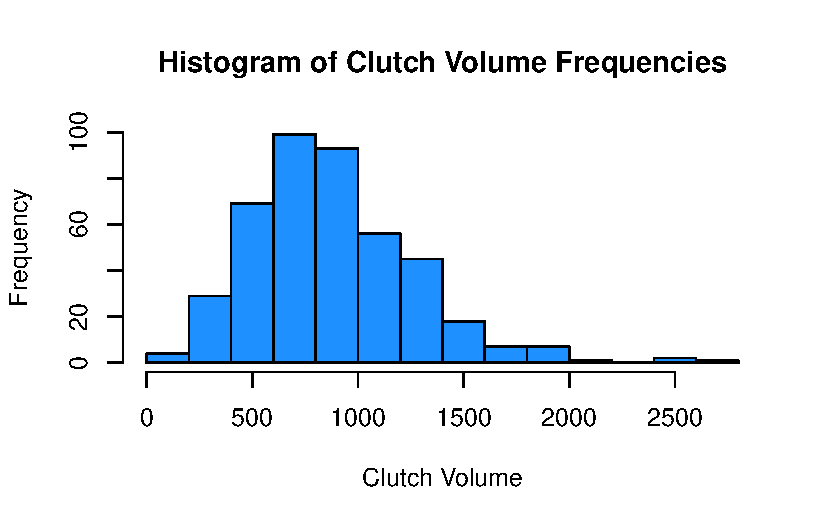
\includegraphics[width=\maxwidth]{figure/unnamed-chunk-24-1} 

\end{knitrout}
\end{centering}

Simplified versions of \textit{OI Biostat} Figures 1.21, 1.22, and 1.23 can also be reproduced using \texttt{plot()}.

\subsection{Correlation}

\textbf{Correlation} is a numerical measure of the strength of a linear relationship. The formula for correlation uses the pairing of the two variables, just as the scatterplot does in a graph, so the data used in calculating correlation is a set of $n$ ordered pairs $(x_1,y_1), (x_2,y_2), \ldots, (x_n, y_n) $.

The correlation between two variables $x$ and $y$ is given by:
		\begin{align*}
          r &=  \frac{1}{n-1}\sum^{n}_{i=1}
          \left(\frac{x_{i}-\overline{x}}
          {s_{x}}\right)\left(\frac{y_{i}-\overline{y}}{s_{y}}\right)
    \end{align*}      
where $(x_1,y_1), (x_2,y_2), \ldots, (x_n, y_n)$ are the $n$ paired values of $x$ and $y$, and $s_x$ and $s_y$ are the sample standard deviations of the $x$ and $y$ variables, respectively.     

The following illustrates the calculations for finding the correlation coefficient of (1,5), (2, 4), and (3,0), as shown in \textit{OI Biostat} Example 1.13.

\begin{knitrout}
\definecolor{shadecolor}{rgb}{0.969, 0.969, 0.969}\color{fgcolor}\begin{kframe}
\begin{alltt}
\hlcom{# define variables}
\hlstd{x} \hlkwb{=} \hlkwd{c}\hlstd{(}\hlnum{1}\hlstd{,} \hlnum{2}\hlstd{,} \hlnum{3}\hlstd{)}
\hlstd{y} \hlkwb{=} \hlkwd{c}\hlstd{(}\hlnum{5}\hlstd{,} \hlnum{4}\hlstd{,} \hlnum{0}\hlstd{)}

\hlcom{# calculate sample means}
\hlstd{x.bar} \hlkwb{=} \hlkwd{mean}\hlstd{(x)}
\hlstd{y.bar} \hlkwb{=} \hlkwd{mean}\hlstd{(y)}

\hlcom{# calculate sample sd's}
\hlstd{sd.x} \hlkwb{=} \hlkwd{sd}\hlstd{(x)}
\hlstd{sd.y} \hlkwb{=} \hlkwd{sd}\hlstd{(y)}

\hlcom{# calculate products and sum of products}
\hlstd{x.component} \hlkwb{=} \hlstd{(x} \hlopt{-} \hlstd{x.bar)}\hlopt{/}\hlstd{(sd.x)}
\hlstd{y.component} \hlkwb{=} \hlstd{(y} \hlopt{-} \hlstd{y.bar)}\hlopt{/}\hlstd{(sd.y)}
\hlstd{products} \hlkwb{=} \hlstd{x.component} \hlopt{*} \hlstd{y.component}
\hlstd{products.sum} \hlkwb{=} \hlkwd{sum}\hlstd{(products)}

\hlcom{# divide by n - 1}
\hlstd{n} \hlkwb{=} \hlkwd{length}\hlstd{(x)}   \hlcom{## n also equals length(y)}
\hlstd{r} \hlkwb{=} \hlstd{products.sum} \hlopt{/} \hlstd{(n} \hlopt{-} \hlnum{1}\hlstd{)}
\hlstd{r}
\end{alltt}
\begin{verbatim}
## [1] -0.9449112
\end{verbatim}
\end{kframe}
\end{knitrout}

It is much easier to use the \texttt{cor()} function to find correlation. 

\begin{knitrout}
\definecolor{shadecolor}{rgb}{0.969, 0.969, 0.969}\color{fgcolor}\begin{kframe}
\begin{alltt}
\hlcom{## Figure 1.22}
\hlkwd{cor}\hlstd{(x,y)}
\end{alltt}
\begin{verbatim}
## [1] -0.9449112
\end{verbatim}
\begin{alltt}
\hlkwd{plot}\hlstd{(x,y)}
\end{alltt}
\end{kframe}
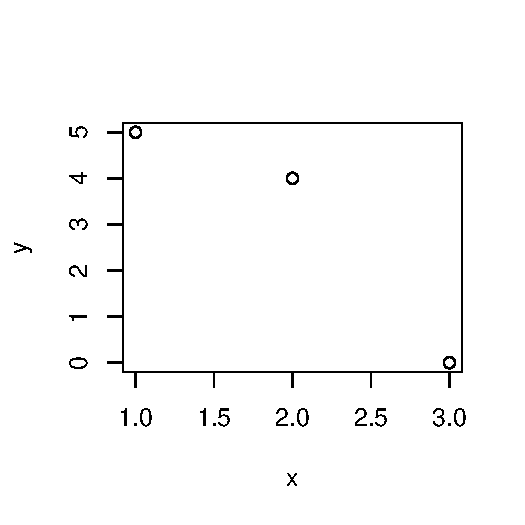
\includegraphics[width=\maxwidth]{figure/unnamed-chunk-26-1} 

\end{knitrout}

The correlation can also be calculated for the income versus life expectancy data plotted in \textit{OI Biostat} Figure 1.23. In this case, the command includes the argument \texttt{use = "complete.obs"} to allow for the computation to disregard any missing values in the dataset.

\begin{knitrout}
\definecolor{shadecolor}{rgb}{0.969, 0.969, 0.969}\color{fgcolor}\begin{kframe}
\begin{alltt}
\hlkwd{cor}\hlstd{(life.expectancy.income}\hlopt{$}\hlstd{income, life.expectancy.income}\hlopt{$}\hlstd{life.expectancy,}
    \hlkwc{use} \hlstd{=} \hlstr{"complete.obs"}\hlstd{)}
\end{alltt}
\begin{verbatim}
## [1] 0.6308783
\end{verbatim}
\end{kframe}
\end{knitrout}

\subsection{Transforming Data}
A \textbf{transformation} is a rescaling of data using a function. The figure below shows the original plot of income data as well as the plot of the log-transformed data. Note that the \texttt{log} command in \textsf{R} computes natural logarithms.

The function \texttt{par()} creates partitions in the graphing output. In this case, specifying \texttt{mfrow = c(1,2)} produces 1 row and 2 columns.

\begin{knitrout}
\definecolor{shadecolor}{rgb}{0.969, 0.969, 0.969}\color{fgcolor}\begin{kframe}
\begin{alltt}
\hlcom{## Figure 1.26}
\hlkwd{par}\hlstd{(}\hlkwc{mfrow} \hlstd{=} \hlkwd{c}\hlstd{(}\hlnum{1}\hlstd{,} \hlnum{2}\hlstd{))}  \hlcom{## this line allows two plots to print at the same time}
\hlkwd{hist}\hlstd{(life.expectancy.income}\hlopt{$}\hlstd{income,} \hlkwc{breaks} \hlstd{=} \hlnum{12}\hlstd{,} \hlkwc{xlab} \hlstd{=} \hlstr{"Income (USD)"}\hlstd{,}
    \hlkwc{ylab} \hlstd{=} \hlstr{"Frequency"}\hlstd{,} \hlkwc{ylim} \hlstd{=} \hlkwd{c}\hlstd{(}\hlnum{0}\hlstd{,} \hlnum{120}\hlstd{),} \hlkwc{main} \hlstd{=} \hlstr{"Untransformed"}\hlstd{)}

\hlkwd{hist}\hlstd{(}\hlkwd{log}\hlstd{(life.expectancy.income}\hlopt{$}\hlstd{income),} \hlkwc{breaks} \hlstd{=} \hlnum{12}\hlstd{,} \hlkwc{xlab} \hlstd{=} \hlstr{"Income (log USD)"}\hlstd{,}
    \hlkwc{ylab} \hlstd{=} \hlstr{"Frequency"}\hlstd{,} \hlkwc{ylim} \hlstd{=} \hlkwd{c}\hlstd{(}\hlnum{0}\hlstd{,} \hlnum{30}\hlstd{),} \hlkwc{main} \hlstd{=} \hlstr{"Log Transformed"}\hlstd{)}
\end{alltt}
\end{kframe}
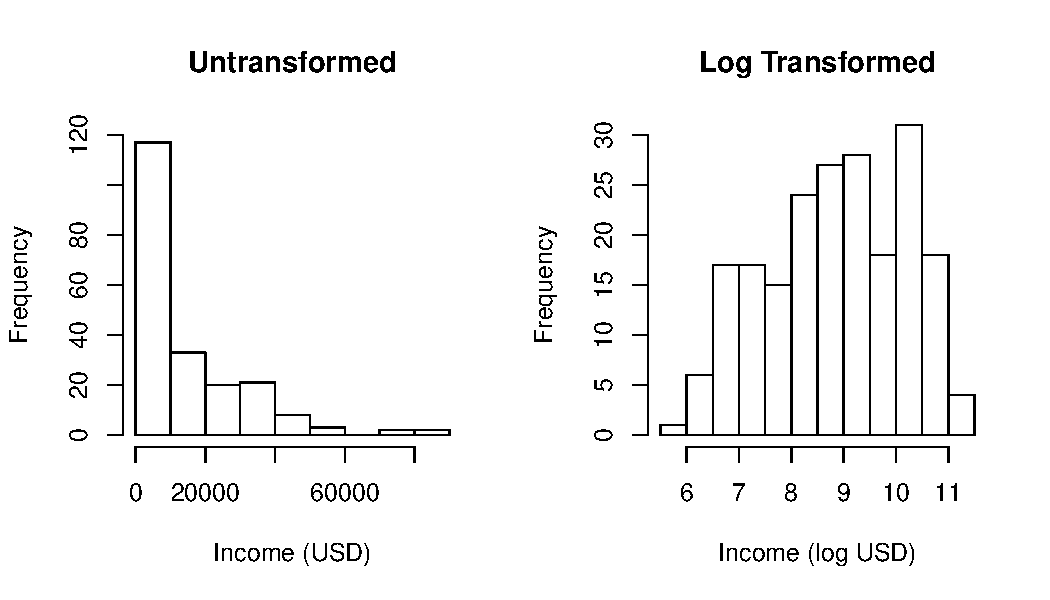
\includegraphics[width=\maxwidth]{figure/unnamed-chunk-28-1} 

\end{knitrout}

Transformations can also be applied to both variables when exploring a relationship. The following figure shows simplified versions of \textit{OI Biostat} Figures 1.23 and 1.27.

\begin{knitrout}
\definecolor{shadecolor}{rgb}{0.969, 0.969, 0.969}\color{fgcolor}\begin{kframe}
\begin{alltt}
\hlcom{## Figure 1.23 and Figure 1.27}
\hlkwd{par}\hlstd{(}\hlkwc{mfrow} \hlstd{=} \hlkwd{c}\hlstd{(}\hlnum{1}\hlstd{,} \hlnum{2}\hlstd{))}
\hlkwd{plot}\hlstd{(life.expectancy.income}\hlopt{$}\hlstd{income, life.expectancy.income}\hlopt{$}\hlstd{life.expectancy,}
    \hlkwc{ylab} \hlstd{=} \hlstr{"Life Expectancy (years)"}\hlstd{,} \hlkwc{xlab} \hlstd{=} \hlstr{"Per Capita Income (USD)"}\hlstd{,}
    \hlkwc{main} \hlstd{=} \hlstr{"Untransformed"}\hlstd{)}
\hlkwd{plot}\hlstd{(}\hlkwd{log}\hlstd{(life.expectancy.income}\hlopt{$}\hlstd{income),} \hlkwd{log}\hlstd{(life.expectancy.income}\hlopt{$}\hlstd{life.expectancy),}
    \hlkwc{ylab} \hlstd{=} \hlstr{"Life Expectancy (log years)"}\hlstd{,} \hlkwc{xlab} \hlstd{=} \hlstr{"Per Capita Income (log USD)"}\hlstd{,}
    \hlkwc{main} \hlstd{=} \hlstr{"Transformed"}\hlstd{)}
\end{alltt}
\end{kframe}
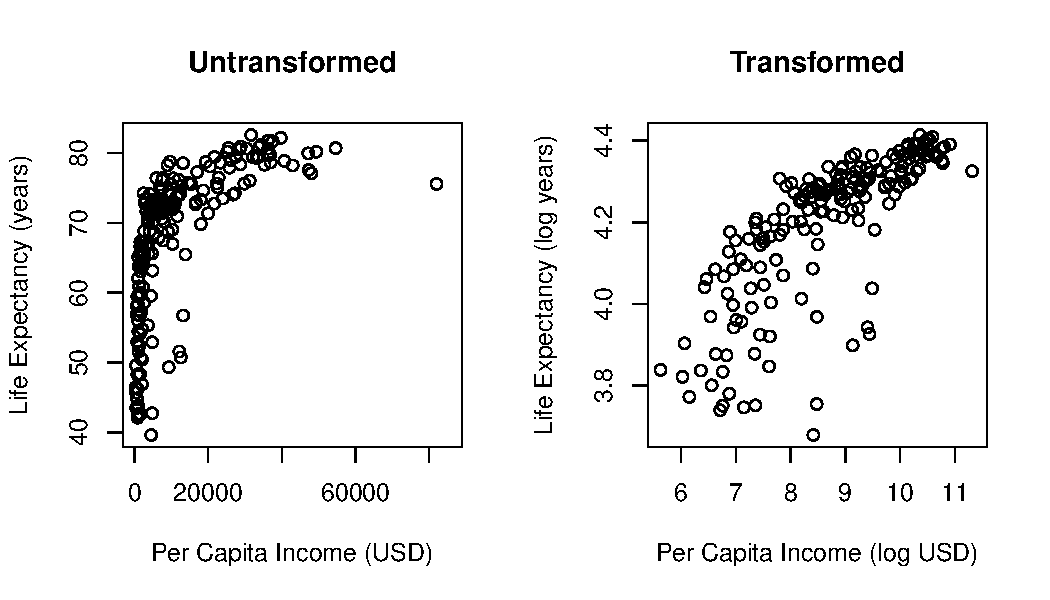
\includegraphics[width=\maxwidth]{figure/unnamed-chunk-29-1} 

\end{knitrout}

\section{Categorical Data}
\subsection{Contingency Tables}

A \textbf{frequency table} shows the counts for each category within a variable. The following \texttt{table()} command produces a frequency table for the \texttt{actn3.r577x} variable.

\begin{knitrout}
\definecolor{shadecolor}{rgb}{0.969, 0.969, 0.969}\color{fgcolor}\begin{kframe}
\begin{alltt}
\hlcom{## Table 1.28}
\hlkwd{addmargins}\hlstd{(}\hlkwd{table}\hlstd{(famuss}\hlopt{$}\hlstd{actn3.r577x))}
\end{alltt}
\begin{verbatim}
## 
##  CC  CT  TT Sum 
## 173 261 161 595
\end{verbatim}
\end{kframe}
\end{knitrout}

A \textbf{contingency table} summarizes data for two categorical variables, such as race and genotype in \textit{OI Biostat} Table 1.29. 

\begin{knitrout}
\definecolor{shadecolor}{rgb}{0.969, 0.969, 0.969}\color{fgcolor}\begin{kframe}
\begin{alltt}
\hlcom{## Table 1.29}
\hlkwd{addmargins}\hlstd{(}\hlkwd{table}\hlstd{(famuss}\hlopt{$}\hlstd{race, famuss}\hlopt{$}\hlstd{actn3.r577x))}
\end{alltt}
\begin{verbatim}
##             
##               CC  CT  TT Sum
##   African Am  16   6   5  27
##   Asian       21  18  16  55
##   Caucasian  125 216 126 467
##   Hispanic     4  10   9  23
##   Other        7  11   5  23
##   Sum        173 261 161 595
\end{verbatim}
\end{kframe}
\end{knitrout}

\textit{OI Biostat} Table 1.30 shows a contingency table with row proportions, computed as the counts divided by their row totals. The \texttt{prop.table()} command produces a table with row proportions, as specified by the \texttt{1} in the argument.

\begin{knitrout}
\definecolor{shadecolor}{rgb}{0.969, 0.969, 0.969}\color{fgcolor}\begin{kframe}
\begin{alltt}
\hlcom{## Table 1.30}
\hlstd{counts.table} \hlkwb{=} \hlkwd{table}\hlstd{(famuss}\hlopt{$}\hlstd{race, famuss}\hlopt{$}\hlstd{actn3.r577x)}
\hlstd{row.prop.table} \hlkwb{=} \hlkwd{prop.table}\hlstd{(counts.table,} \hlnum{1}\hlstd{)}
\hlstd{row.prop.table}
\end{alltt}
\begin{verbatim}
##             
##                     CC        CT        TT
##   African Am 0.5925926 0.2222222 0.1851852
##   Asian      0.3818182 0.3272727 0.2909091
##   Caucasian  0.2676660 0.4625268 0.2698073
##   Hispanic   0.1739130 0.4347826 0.3913043
##   Other      0.3043478 0.4782609 0.2173913
\end{verbatim}
\end{kframe}
\end{knitrout}

Alternatively, a contingency table can be created with column proportions by changing the \texttt{1} in \texttt{prop.table()} to a \texttt{2}. 

\begin{knitrout}
\definecolor{shadecolor}{rgb}{0.969, 0.969, 0.969}\color{fgcolor}\begin{kframe}
\begin{alltt}
\hlcom{## Table 1.31}
\hlstd{counts.table} \hlkwb{=} \hlkwd{table}\hlstd{(famuss}\hlopt{$}\hlstd{race, famuss}\hlopt{$}\hlstd{actn3.r577x)}
\hlstd{col.prop.table} \hlkwb{=} \hlkwd{prop.table}\hlstd{(counts.table,} \hlnum{2}\hlstd{)}
\hlstd{col.prop.table}
\end{alltt}
\begin{verbatim}
##             
##                      CC         CT         TT
##   African Am 0.09248555 0.02298851 0.03105590
##   Asian      0.12138728 0.06896552 0.09937888
##   Caucasian  0.72254335 0.82758621 0.78260870
##   Hispanic   0.02312139 0.03831418 0.05590062
##   Other      0.04046243 0.04214559 0.03105590
\end{verbatim}
\end{kframe}
\end{knitrout}

\subsection{Bar Plots}

A \textbf{bar plot} is a common way to display a single categorical variable, either from count data or from proportions. The \texttt{barplot()} command requires values to be input in a table format. In the below example, the \texttt{table()} command is nested within the \texttt{barplot()} command.

\begin{knitrout}
\definecolor{shadecolor}{rgb}{0.969, 0.969, 0.969}\color{fgcolor}\begin{kframe}
\begin{alltt}
\hlcom{## Figure 1.32}
\hlkwd{par}\hlstd{(}\hlkwc{mfrow} \hlstd{=} \hlkwd{c}\hlstd{(}\hlnum{1}\hlstd{,} \hlnum{2}\hlstd{))}
\hlkwd{barplot}\hlstd{(}\hlkwd{table}\hlstd{(famuss}\hlopt{$}\hlstd{actn3.r577x))}  \hlcom{## count barplot}
\hlkwd{barplot}\hlstd{(}\hlkwd{table}\hlstd{(famuss}\hlopt{$}\hlstd{actn3.r577x)}\hlopt{/}\hlkwd{sum}\hlstd{(}\hlkwd{table}\hlstd{(famuss}\hlopt{$}\hlstd{actn3.r577x)))}  \hlcom{## frequency barplot}
\end{alltt}
\end{kframe}
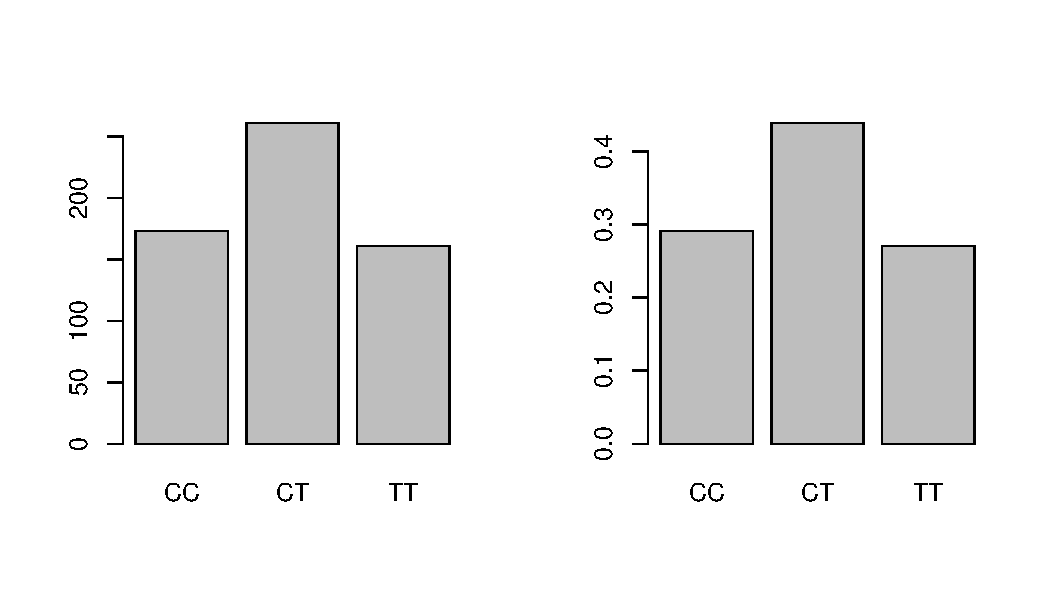
\includegraphics[width=\maxwidth]{figure/unnamed-chunk-34-1} 

\end{knitrout}

\newpage

\subsection{Segmented Bar Plot}

A \textbf{segmented bar plot} draws from a contingency table to display information about two categorical variables. The following code reproduces \textit{OI Biostat} Figure 1.33a, in which a bar plot was created using the \texttt{actn3.r577x} variable, with each group divided by the levels of race. The simplified version of the plot uses the default greyscale shading; it is also possible to specify a list of colors using \texttt{c()}. 

The argument \texttt{legend} can be used to specify whether the row names or the column names are used for the legend. 

\begin{knitrout}
\definecolor{shadecolor}{rgb}{0.969, 0.969, 0.969}\color{fgcolor}\begin{kframe}
\begin{alltt}
\hlcom{## Figure 1.31a}
\hlstd{counts.table} \hlkwb{=} \hlstd{(}\hlkwd{table}\hlstd{(famuss}\hlopt{$}\hlstd{race, famuss}\hlopt{$}\hlstd{actn3.r577x))}
\hlkwd{barplot}\hlstd{(counts.table,} \hlkwc{legend} \hlstd{=} \hlkwd{rownames}\hlstd{(counts.table))}
\end{alltt}
\end{kframe}
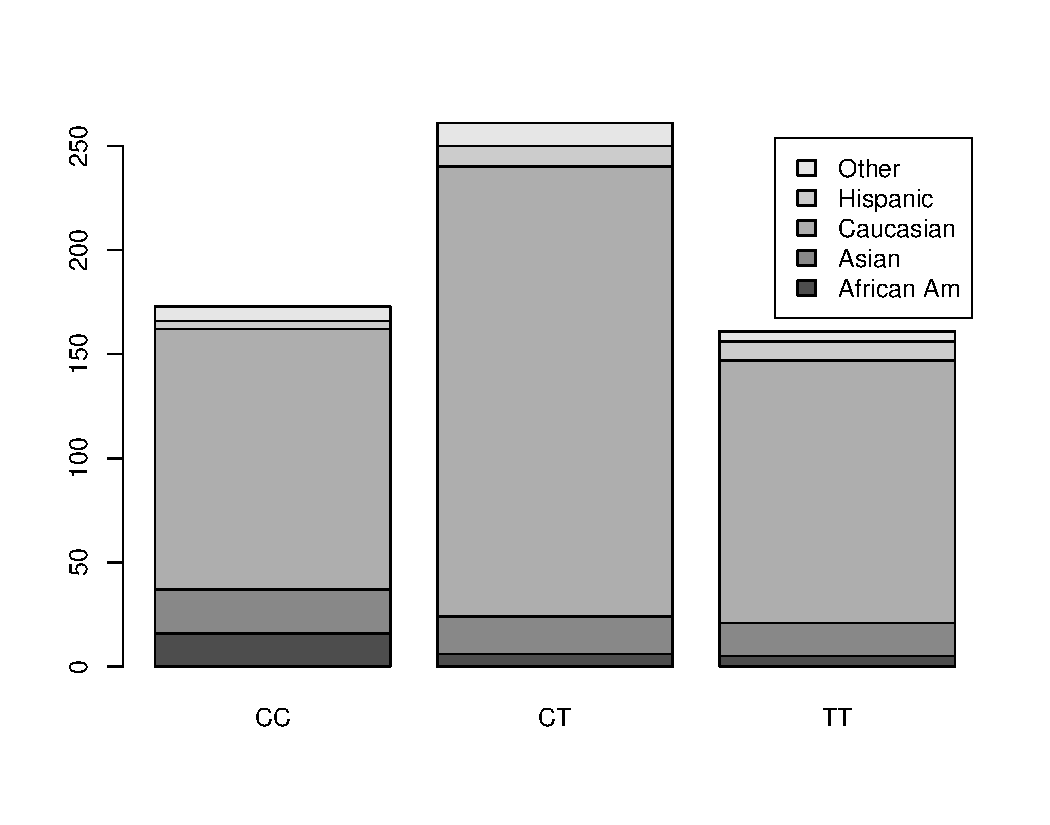
\includegraphics[width=\maxwidth]{figure/unnamed-chunk-35-1} 
\begin{kframe}\begin{alltt}
\hlkwd{barplot}\hlstd{(counts.table,} \hlkwc{col} \hlstd{=} \hlkwd{c}\hlstd{(}\hlstr{"gray"}\hlstd{,} \hlstr{"firebrick1"}\hlstd{,} \hlstr{"dodgerblue"}\hlstd{,}
    \hlstr{"darkgreen"}\hlstd{,} \hlstr{"gold"}\hlstd{),} \hlkwc{ylim} \hlstd{=} \hlkwd{c}\hlstd{(}\hlnum{0}\hlstd{,} \hlnum{300}\hlstd{),} \hlkwc{legend} \hlstd{=} \hlkwd{rownames}\hlstd{(counts.table))}
\end{alltt}
\end{kframe}
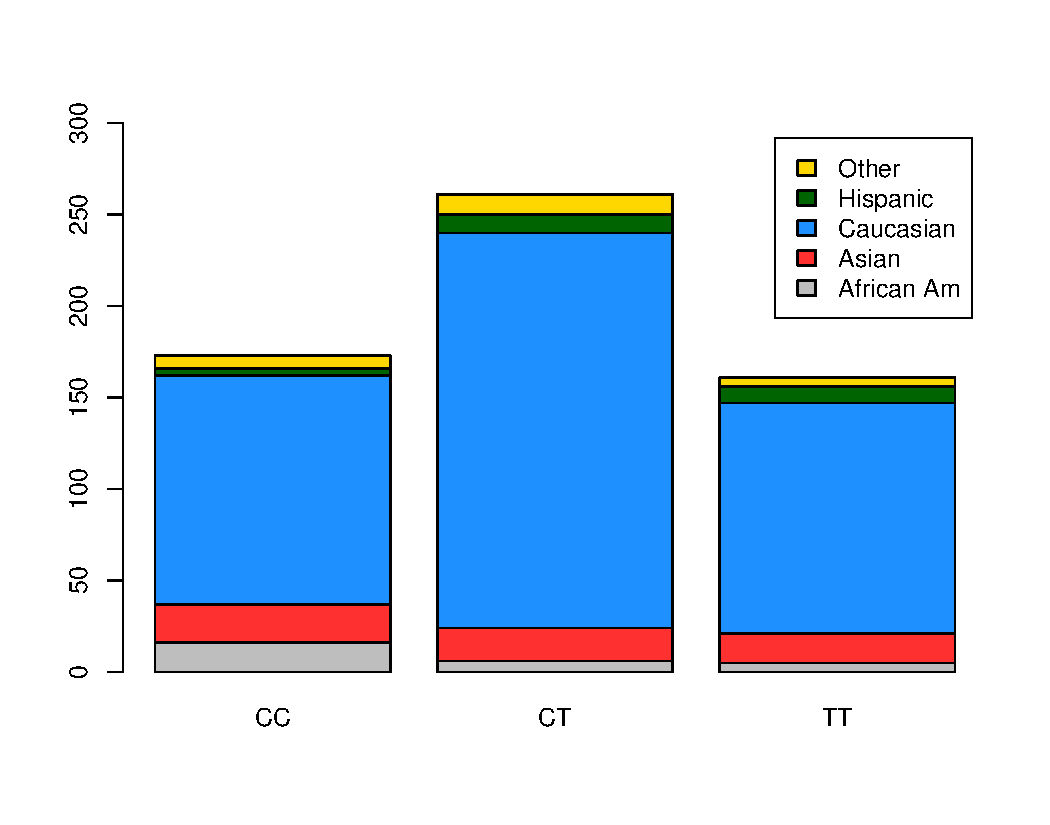
\includegraphics[width=\maxwidth]{figure/unnamed-chunk-35-2} 

\end{knitrout}


%<<tidy = TRUE, fig.height=5, tidy.opts=list(width.cutoff=60)>>=
%## Figure 1.31a
%# first, create a table of the data that is sorted
%genotype.race = matrix(table(famuss$actn3.r577x, famuss$race), ncol=3, byrow=T)

%# second, change the column and row names on the table
%colnames(genotype.race)=c("CC", "CT", "TT")
%rownames(genotype.race)=c("African Am", "Asian", "Caucasian", "Hispanic", "Other")

%# third, plot the barplot where colors are specified
%barplot(genotype.race, col=c("grey", "red", "blue", "green", "yellow"), ylim=
%          c(0,300), width=2)
%# lastly, include a legend for intepretation of your plots
%legend("topright", inset=c(.05, 0), fill=c("grey", "red", "blue", "green", "yellow"),
%       legend=rownames(genotype.race))
%@

\newpage

A \textbf{standardized segmented bar plot} uses proportions to scale the data, and draws from a contingency table with proportions. Setting \texttt{ylim} from 0 to 1.7 allows for enough empty space on the plot so that the legend does not overlap the bars.

\begin{knitrout}
\definecolor{shadecolor}{rgb}{0.969, 0.969, 0.969}\color{fgcolor}\begin{kframe}
\begin{alltt}
\hlcom{## Figure 1.33b}
\hlstd{counts.table} \hlkwb{=} \hlstd{(}\hlkwd{table}\hlstd{(famuss}\hlopt{$}\hlstd{race, famuss}\hlopt{$}\hlstd{actn3.r577x))}
\hlstd{row.prop.table} \hlkwb{=} \hlkwd{prop.table}\hlstd{(counts.table,} \hlnum{2}\hlstd{)}
\hlkwd{barplot}\hlstd{(row.prop.table,} \hlkwc{ylim} \hlstd{=} \hlkwd{c}\hlstd{(}\hlnum{0}\hlstd{,} \hlnum{1.7}\hlstd{),} \hlkwc{legend} \hlstd{=} \hlkwd{rownames}\hlstd{(counts.table))}
\end{alltt}
\end{kframe}
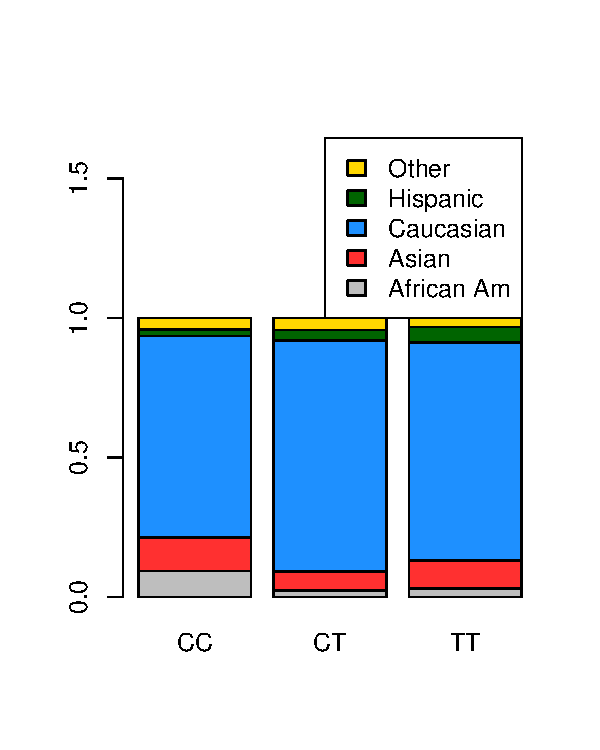
\includegraphics[width=\maxwidth]{figure/unnamed-chunk-36-1} 
\begin{kframe}\begin{alltt}
\hlkwd{barplot}\hlstd{(row.prop.table,} \hlkwc{col} \hlstd{=} \hlkwd{c}\hlstd{(}\hlstr{"gray"}\hlstd{,} \hlstr{"firebrick1"}\hlstd{,} \hlstr{"dodgerblue"}\hlstd{,}
    \hlstr{"darkgreen"}\hlstd{,} \hlstr{"gold"}\hlstd{),} \hlkwc{ylim} \hlstd{=} \hlkwd{c}\hlstd{(}\hlnum{0}\hlstd{,} \hlnum{1.7}\hlstd{),} \hlkwc{legend} \hlstd{=} \hlkwd{rownames}\hlstd{(counts.table))}
\end{alltt}
\end{kframe}
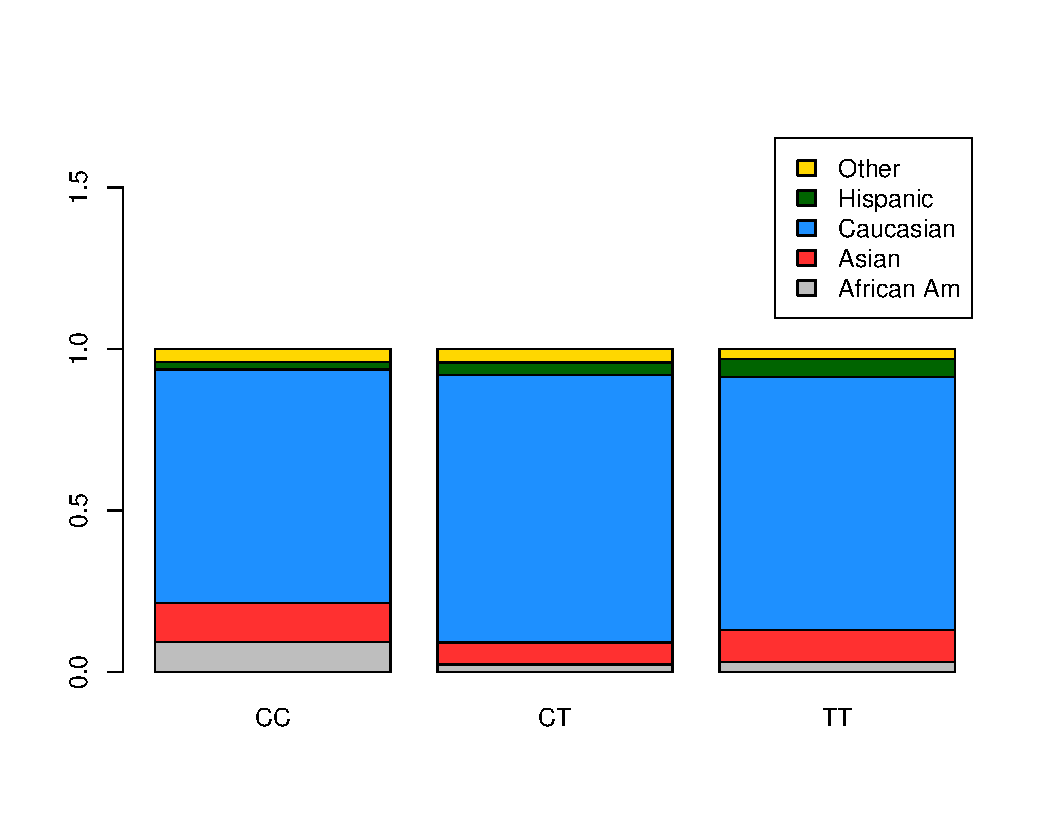
\includegraphics[width=\maxwidth]{figure/unnamed-chunk-36-2} 

\end{knitrout}

%<<tidy = TRUE, fig.height=5, tidy.opts=list(width.cutoff=60)>>=
%## Figure 1.31b
%# first, create table of proportions
%prop.genotype.race <- prop.table(genotype.race, 2)
%
%# second, change the column and row names on the table
%colnames(prop.genotype.race)=c("CC", "CT", "TT")
%rownames(prop.genotype.race)=c("African Am", "Asian", "Caucasian", "Hispanic", "Other")
%
%#second, plot the output
%barplot(prop.genotype.race, col=c("grey", "red", "blue", "green", "yellow"),
%        ylim=c(0, 1.5), width=2)

%# lastly, include a legend for intepretation of your plots
%legend("topright", inset=c(0.05, -0.005), fill=c("grey", "red", "blue", "green", "yellow"),
%       legend=rownames(prop.genotype.race), bty = "n")
%@
%\textit{Note:} In the \textit{legend} line, the command  \textit{inset=} controls where on the plot the legend prints out.  Sometimes this specification can be a little bit bizarre so it may require some alteration to find the right spot for the legend.  

In \textit{OI Biostat} Figure 1.34, the data from the contingency table are organized differently, with each bar representing a level of \texttt{race}. To make this change, reverse the order of the variables in \texttt{counts.table}

\begin{knitrout}
\definecolor{shadecolor}{rgb}{0.969, 0.969, 0.969}\color{fgcolor}\begin{kframe}
\begin{alltt}
\hlcom{## Figure 1.34a}
\hlstd{counts.table} \hlkwb{=} \hlstd{(}\hlkwd{table}\hlstd{(famuss}\hlopt{$}\hlstd{actn3.r577x, famuss}\hlopt{$}\hlstd{race))}  \hlcom{## change variable order}

\hlkwd{barplot}\hlstd{(counts.table,} \hlkwc{col} \hlstd{=} \hlkwd{c}\hlstd{(}\hlstr{"dodgerblue"}\hlstd{,} \hlstr{"darkgreen"}\hlstd{,} \hlstr{"gold"}\hlstd{),}
    \hlkwc{ylim} \hlstd{=} \hlkwd{c}\hlstd{(}\hlnum{0}\hlstd{,} \hlnum{500}\hlstd{),} \hlkwc{legend} \hlstd{=} \hlkwd{rownames}\hlstd{(counts.table))}
\end{alltt}
\end{kframe}
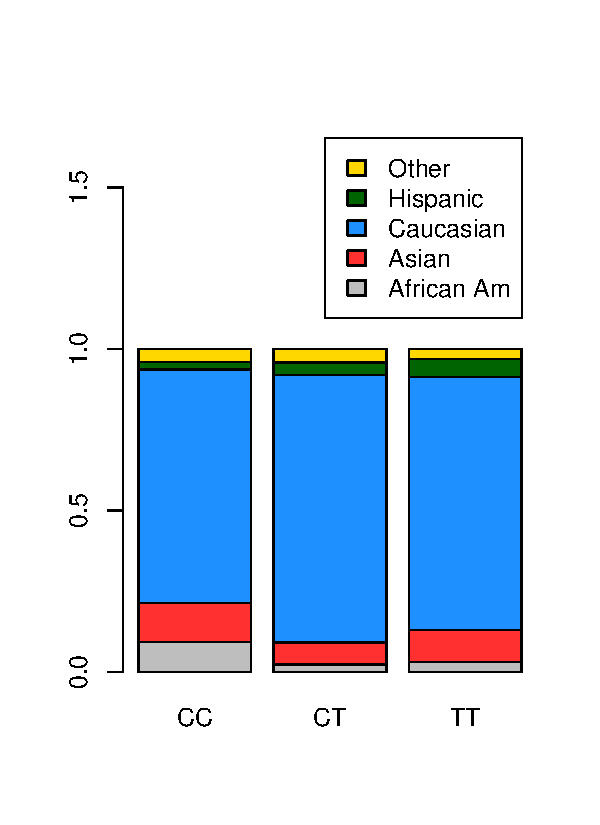
\includegraphics[width=\maxwidth]{figure/unnamed-chunk-37-1} 
\begin{kframe}\begin{alltt}
\hlcom{## Figure 1.34b}
\hlstd{row.prop.table} \hlkwb{=} \hlkwd{prop.table}\hlstd{(counts.table,} \hlnum{2}\hlstd{)}
\hlkwd{barplot}\hlstd{(row.prop.table,} \hlkwc{col} \hlstd{=} \hlkwd{c}\hlstd{(}\hlstr{"dodgerblue"}\hlstd{,} \hlstr{"darkgreen"}\hlstd{,} \hlstr{"gold"}\hlstd{),}
    \hlkwc{ylim} \hlstd{=} \hlkwd{c}\hlstd{(}\hlnum{0}\hlstd{,} \hlnum{1.8}\hlstd{),} \hlkwc{legend} \hlstd{=} \hlkwd{rownames}\hlstd{(counts.table))}
\end{alltt}
\end{kframe}
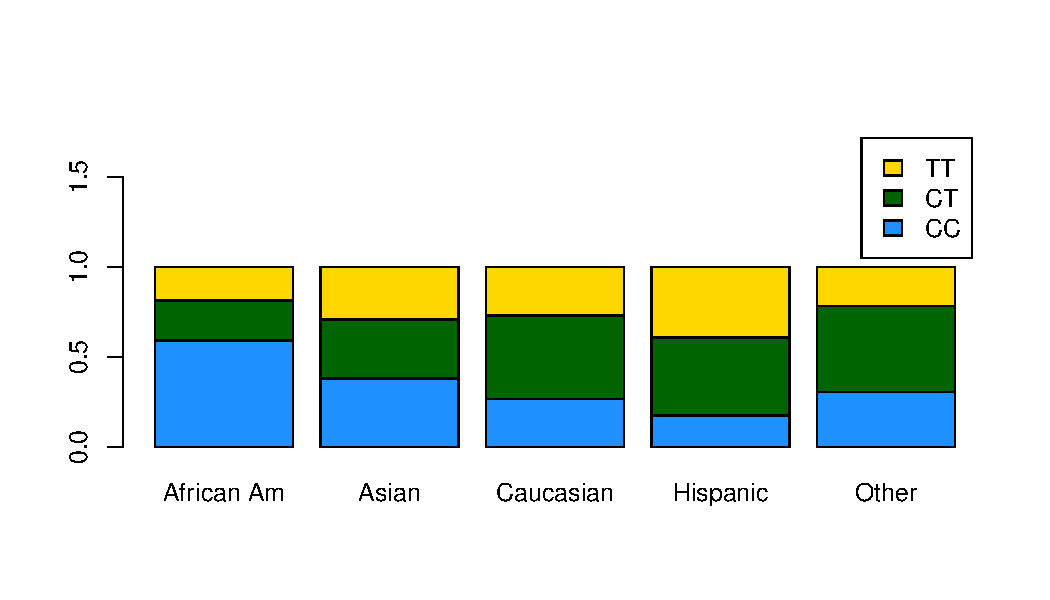
\includegraphics[width=\maxwidth]{figure/unnamed-chunk-37-2} 

\end{knitrout}

%If we wanted to reproduce Figure 1.32, where the bars indicate race instead of %genotype, we can do the same process as above, with one exception.  In the first step, %of creating the table, we must instead put the race variable first as the rows and the %gene variable as the columns, as follows:
%<<tidy = TRUE, fig.height=4, tidy.opts=list(width.cutoff=60)>>=
%## Figure 1.32
%# Plotting two graphs next to each other
%par(mfrow=(c(1,2)))
%
%# Setting up the table and changing column/row names
%race.genotype = matrix(table(famuss$race, famuss$actn3.r577x), ncol=5, byrow=T)
%colnames(race.genotype)=c("African Am", "Asian", "Caucasian", "Hispanic", "Other")
%rownames(race.genotype)=c("CC", "CT", "TT")
%
%# Creating segmented bar plot with a legend
%barplot(race.genotype, col=c("blue", "green", "yellow"), ylim=c(0,500), width=2)
%legend("topright", inset=c(0, 0), fill=c("blue", "green", "yellow"), 
%      legend=rownames(race.genotype))
%
%# Creating standardized segmented bar plot with a legend
%prop.race.genotype <- prop.table(race.genotype, 2)
%barplot(prop.race.genotype, col=c("blue", "green", "yellow"), ylim=c(0, 1.5), width=2)
%legend("topright", inset=c(0, 0), fill=c("blue", "green", "yellow"), 
%       legend=rownames(race.genotype))
%@

\subsection{Comparing numerical data across groups}
\subsubsection{Side-by-side boxplots}

The \textbf{side-by-side} boxplot is a useful tool for comparing the distribution of numerical data across categories. \textit{OI Biostat} Figure 1.35a shows a side-by-side boxplot for percent change in non-dominant arm strength grouped by genotype. The response variable $y$ comes before the tilde and the explanatory variable $x$; in this case, the response variable is percent change in strength.

\begin{knitrout}
\definecolor{shadecolor}{rgb}{0.969, 0.969, 0.969}\color{fgcolor}\begin{kframe}
\begin{alltt}
\hlcom{## Figure 1.335(a)}
\hlkwd{boxplot}\hlstd{(famuss}\hlopt{$}\hlstd{ndrm.ch} \hlopt{~} \hlstd{famuss}\hlopt{$}\hlstd{actn3.r577x,}
    \hlkwc{ylab} \hlstd{=} \hlstr{"% Change in Non-Dominant Arm Strength"}\hlstd{,}
    \hlkwc{xlab} \hlstd{=} \hlstr{"Genotype"}\hlstd{)}
\end{alltt}
\end{kframe}
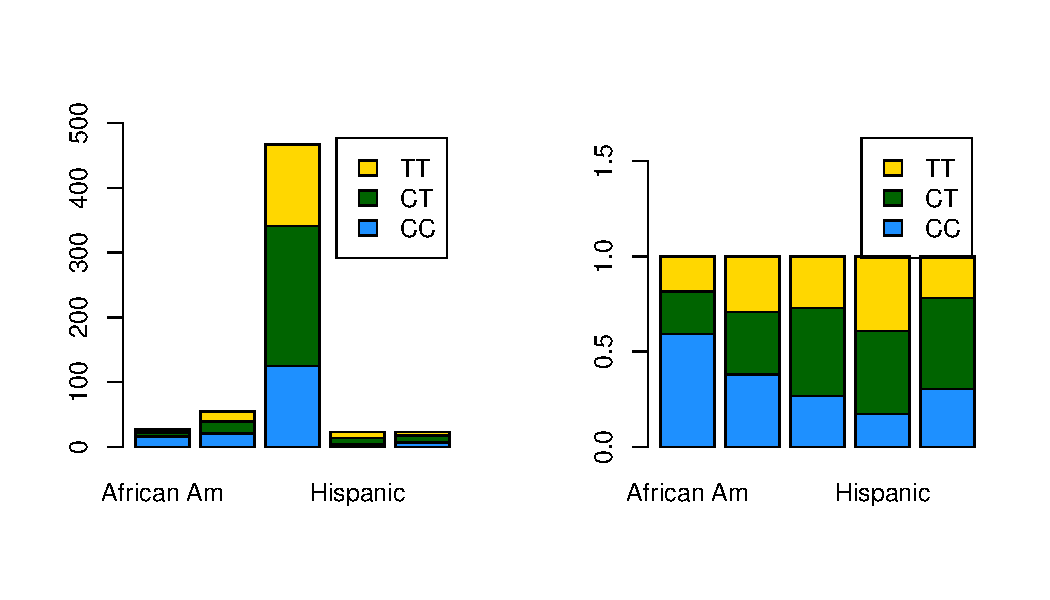
\includegraphics[width=\maxwidth]{figure/unnamed-chunk-38-1} 

\end{knitrout}

\textit{OI Biostat} Figure 1.36 shows a larger side-by-side boxplot which compares the distribution of frog clutch sizes for different altitudes.

\begin{knitrout}
\definecolor{shadecolor}{rgb}{0.969, 0.969, 0.969}\color{fgcolor}\begin{kframe}
\begin{alltt}
\hlcom{## Figure 1.36}
\hlkwd{boxplot}\hlstd{(frog.altitude.data}\hlopt{$}\hlstd{clutch.volume} \hlopt{~} \hlstd{frog.altitude.data}\hlopt{$}\hlstd{altitude,}
    \hlkwc{xlab} \hlstd{=} \hlstr{"Clutch Volume"}\hlstd{,} \hlkwc{ylab} \hlstd{=} \hlstr{"Altitude"}\hlstd{)}
\end{alltt}
\end{kframe}
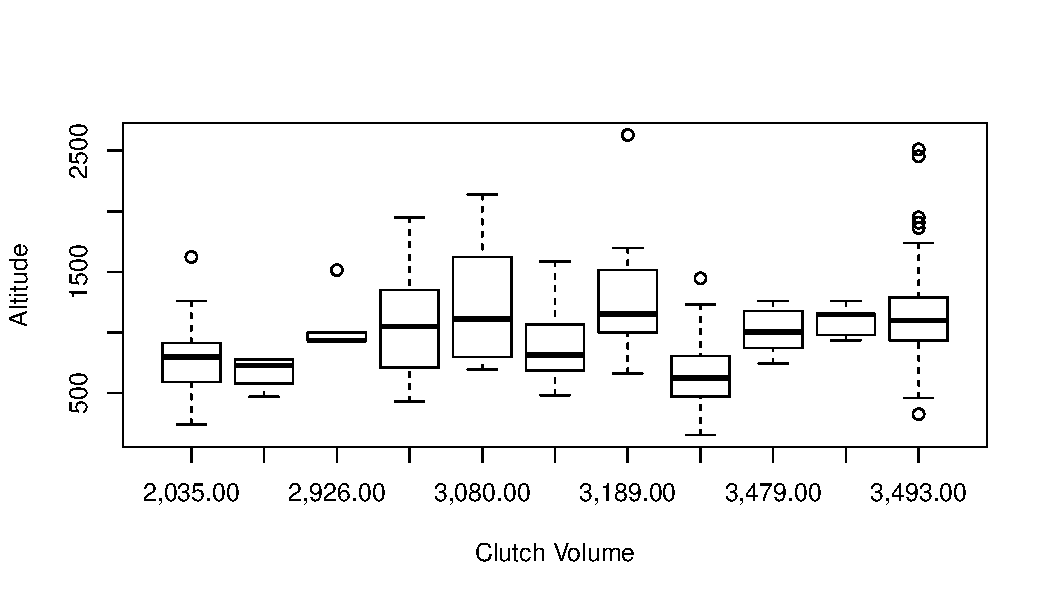
\includegraphics[width=\maxwidth]{figure/unnamed-chunk-39-1} 

\end{knitrout}

\subsubsection{Hollow Histograms}

A \textbf{hollow histogram} plots the outlines of histograms for each group onto the same axes. To plot a hollow histogram, specify any axis limits and labels in the command for the first histogram; the subsequent histograms require the argument \texttt{add = T} in order for them to be overlaid on top of the first plot.

\begin{knitrout}
\definecolor{shadecolor}{rgb}{0.969, 0.969, 0.969}\color{fgcolor}\begin{kframe}
\begin{alltt}
\hlcom{## Figure 1.35(b)}
\hlkwd{hist}\hlstd{(famuss}\hlopt{$}\hlstd{ndrm.ch[famuss}\hlopt{$}\hlstd{actn3.r577x} \hlopt{==} \hlstr{"CC"}\hlstd{],} \hlkwc{breaks} \hlstd{=} \hlnum{20}\hlstd{,} \hlkwc{border} \hlstd{=} \hlstr{"dodgerblue"}\hlstd{,}
     \hlkwc{xlab} \hlstd{=} \hlstr{"% Change in Non-Dominant Arm Strength"}\hlstd{,} \hlkwc{ylim} \hlstd{=} \hlkwd{c}\hlstd{(}\hlnum{0}\hlstd{,}\hlnum{50}\hlstd{),} \hlkwc{xlim} \hlstd{=} \hlkwd{c}\hlstd{(}\hlnum{0}\hlstd{,}\hlnum{250}\hlstd{),}
     \hlkwc{main} \hlstd{=} \hlstr{"Percent Change in Non-Dominant Arm Strength by Genotype"}\hlstd{)}
\hlkwd{hist}\hlstd{(famuss}\hlopt{$}\hlstd{ndrm.ch[famuss}\hlopt{$}\hlstd{actn3.r577x} \hlopt{==} \hlstr{"CT"}\hlstd{],} \hlkwc{breaks} \hlstd{=} \hlnum{20}\hlstd{,} \hlkwc{border} \hlstd{=} \hlstr{"darkgreen"}\hlstd{,}
     \hlkwc{add} \hlstd{= T)}
\hlkwd{hist}\hlstd{(famuss}\hlopt{$}\hlstd{ndrm.ch[famuss}\hlopt{$}\hlstd{actn3.r577x} \hlopt{==} \hlstr{"TT"}\hlstd{],} \hlkwc{breaks} \hlstd{=} \hlnum{20}\hlstd{,} \hlkwc{border} \hlstd{=} \hlstr{"firebrick1"}\hlstd{,}
     \hlkwc{add} \hlstd{= T)}

\hlkwd{legend}\hlstd{(}\hlstr{'topright'}\hlstd{,}
       \hlkwc{col} \hlstd{=} \hlkwd{c}\hlstd{(}\hlstr{"dodgerblue"}\hlstd{,} \hlstr{"darkgreen"}\hlstd{,} \hlstr{"firebrick1"}\hlstd{),}
       \hlkwc{lwd} \hlstd{=} \hlkwd{c}\hlstd{(}\hlnum{1}\hlstd{,} \hlnum{1}\hlstd{,} \hlnum{1}\hlstd{),}     \hlcom{## line width}
       \hlkwc{legend} \hlstd{=} \hlkwd{c}\hlstd{(}\hlstr{'CC'}\hlstd{,} \hlstr{'CT'}\hlstd{,} \hlstr{'TT'}\hlstd{))}    \hlcom{##legend labels}
\end{alltt}
\end{kframe}
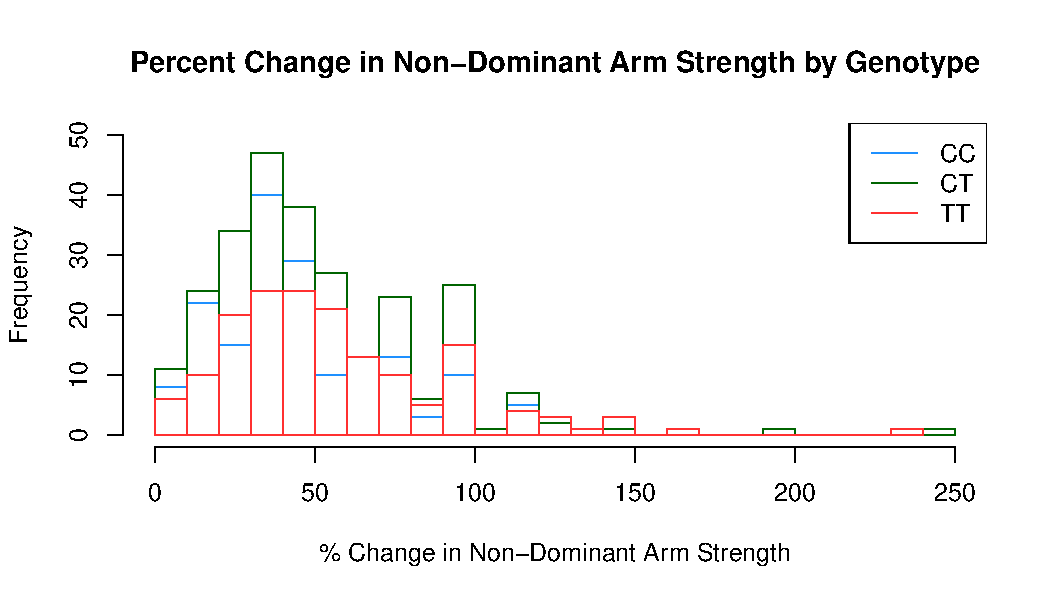
\includegraphics[width=\maxwidth]{figure/unnamed-chunk-40-1} 

\end{knitrout}

\section{Genomic Data}

% JV: Golub data (golub_exprs_pheno) needs to be added to the package

% JV: Add material from 102 section 2 to this section, as an exercise? Doesn't seem useful to just reproduce the figures in OI Biostat 1.6 here.

\begin{knitrout}
\definecolor{shadecolor}{rgb}{0.969, 0.969, 0.969}\color{fgcolor}\begin{kframe}
\begin{alltt}
\hlkwd{boxplot}\hlstd{(golub.exprs.pheno[,} \hlnum{7}\hlopt{:}\hlnum{9}\hlstd{])}
\end{alltt}


{\ttfamily\noindent\bfseries\color{errorcolor}{\#\# Error in boxplot(golub.exprs.pheno[, 7:9]): object 'golub.exprs.pheno' not found}}\end{kframe}
\end{knitrout}


\newpage 
\chapter{Using R for Probabilities}
\minitoc

\vspace{0.5cm} 

This chapter focuses on the material covered in \textit{OI Biostat} Chapter 2, Section 2.5. While simple conditional probability problems are easily solved by hand with a basic calculator, \textsf{R} can be useful for more elaborate scenarios like those that involve Bayes' Theorem.

What are the chances that a woman with a positive mamogram has breast cancer? This question can be rephrased as the conditional probability that a woman has breast cancer, given that her mammogram is abnormal, otherwise known as the \textbf{positive predictive value} of a mammogram. Two methods discussed in this chapter, using Bayes' Theorem and creating a contingency table, are also explained in \textit{OI Biostat}. This chapter will also cover an additional approach: modeling the problem scenario by running a simulation.

\begin{quotation}

\textbf{\textit{OI Biostat} Example 2.37.} In Canada, about 0.35\% of women over 40 will develop breast cancer in any given year. A common screening test for cancer is the mammogram, but it is not perfect. In about 11\% of patients with breast cancer, the test gives a \textbf{false negative}: it indicates a woman does not have breast cancer when she does have breast cancer. Similarly, the test gives a \textbf{false positive} in 7\% of patients who do not have breast cancer: it indicates these patients have breast cancer when they actually do not. If a randomly selected woman over 40 is tested for breast cancer using a mammogram and the test is positive -- that is, the test suggests the woman has cancer -- what is the probability she has breast cancer?

\end{quotation}

%Chapter 2 explains probability, how its used, and what questions it can be used to answer.  In this chapter, we will go through some examples of how \texttt{R} can be used to solve propability problems.  Once again, we will see that there are several different methods that can be used to answer the same question.  

%We will focus on \textbf{conditional probability} here as these are the questions you would most commonly use \texttt{R} to solve.  To review, a conditional probability is the probability of an outcome given prior knowledge about another factor or condition.  For example, we could ask what is the conditional probability of an individual being male \textit{given} they have brown hair.  \textbf{Joint probability} is the probability of two events occuring simultaneously.  Referring back to our example, the joint probability would be the probability of an individual being male \textit{and} having brown hair.  We could also consider the \textbf{marginal probability}, or the probability of a single event occuring, such as an individual being male.  Another marginal probability would be the probability of an individual having brown hair.  

%The mathematical definition for conditional probability is, for events \textit{A} and \textit{B}, the probability of \textit{A} given \textit{B} is computed as 
%$$ P(A|B) = \frac{P(A \textnormal{ and } B)}{P(B)} $$

%\section{Case Study on Conditional Probability}
%In order to demonstrate the various techniques which can be used to solve a conditional probability question in R, we are going to consider a case study of cystic fibrosis.  The prevalence of cystic fibrosis is considered to be 1 in 6000 people.  A test used to screen for cystic fibrosis has a \textbf{sensitivity} of 0.950, meaning that it correctly gives a positive test result in a patient with the disease 95\% of the time.  This can also be referred to as the \textbf{true positive rate}.  Additionally, the test has a \textbf{specificity} of 0.99897, meaning that it correctly gives a negative test result in a patient without the disease 99.897\% of the time.  This can be referred to as the \textbf{true negative rate}.  Using this information, we want to determine the \textbf{positive predictive value} of the test, or the probability of a patient having the disease given their test result is positive.  

% JV: I think it will be helpful to show exactly the example done in the text, since a new method (simulation) is being introduced in this chapter.

\section{Bayes' Theorem}

Bayes' Theorem states that the conditional probability $P(A_1 | B)$ can be identified as the following fraction:\vspace{-1.5mm}
\begin{align*}
\frac{P(A_1 \text{and } B)}{P(B)}= \frac{P(B | A_1) P(A_1)}
	{P(B | A_1) P(A_1) + P(B | A_2) P(A_2) + \cdots + P(B | A_k) P(A_k)}
\end{align*}
where $A_2$, $A_3$, ..., and $A_k$ represent all other possible outcomes of the first variable.

The expression can also be written in terms of diagnostic testing language, where $D = \text{\{has disease\}}$, $D^c = \text{\{does not have disease\}}$, $T^{+} = \text{\{positive test result\}}$, and $T^{-} = \text{\{negative test result\}}$.

\begin{align*}
P(D|T^{+}) &= \dfrac{P(D \text{ and } T^{+})}{P(D)} \\
&= \dfrac{P(T^{+}|D) \times P(D)}{[P(T^{+}|D) \times P(D)] + [P(T^{+}|D^c) \times P(D^c)]} \\
\text{PPV} &= \dfrac{\text{sensitivity } \times \text{ prevalence}}{[\text{sensitivity } \times \text{ prevalence}] + [\text{(1 - specificity) } \times \text{ (1 - prevalence)}]}
\end{align*}

\textsf{R} can be used to store values for prevalence, sensitivity, and specificity so that calculations are less tedious. Recall that the \textbf{sensitivity} is the probability of a positive test result when disease is present, which is the complement of a false negative. The \textbf{specificity} is the probability of a negative test result when disease is absent, which is the complement of a false positive.

\begin{knitrout}
\definecolor{shadecolor}{rgb}{0.969, 0.969, 0.969}\color{fgcolor}\begin{kframe}
\begin{alltt}
\hlstd{prevalence} \hlkwb{=} \hlnum{0.0035}
\hlstd{sensitivity} \hlkwb{=} \hlnum{1} \hlopt{-} \hlnum{0.11}
\hlstd{specificity} \hlkwb{=} \hlnum{1} \hlopt{-} \hlnum{0.07}

\hlstd{ppv.num} \hlkwb{=} \hlstd{(sensitivity}\hlopt{*}\hlstd{prevalence)}  \hlcom{## numerator}
\hlstd{ppv.den} \hlkwb{=} \hlstd{ppv.num} \hlopt{+} \hlstd{((}\hlnum{1}\hlopt{-}\hlstd{specificity)}\hlopt{*}\hlstd{(}\hlnum{1}\hlopt{-}\hlstd{prevalence))}  \hlcom{## denominator}
\hlstd{ppv} \hlkwb{=} \hlstd{ppv.num} \hlopt{/} \hlstd{ppv.den}

\hlstd{ppv}
\end{alltt}
\begin{verbatim}
## [1] 0.04274736
\end{verbatim}
\end{kframe}
\end{knitrout}


\section{Contingency Table}

The PPV can also be calculated by constructing a two-way contingency table for a hypothetical population and calculating conditional probabilities by conditioning on rows or columns. While this method results in an estimate of PPV, using a large enough population size such as 100,000 produces an empirical estimate that is very close to the exact value found through using Bayes' Theorem. 

\begin{center}
\begin{tabular}{|l|c|c|r|}
\hline 
& D+ & D- & Total\\ 
\hline
T+ & & & \\ 
\hline
T- & & & \\ 
\hline 
Total & & & 100,000 \\ 
\hline 
\end{tabular} 
\end{center} 

First, calculate the expected number of disease cases and non-disease cases in the population:
\begin{knitrout}
\definecolor{shadecolor}{rgb}{0.969, 0.969, 0.969}\color{fgcolor}\begin{kframe}
\begin{alltt}
\hlstd{population.size} \hlkwb{=} \hlnum{100000}
\hlstd{expected.cases} \hlkwb{=} \hlstd{prevalence} \hlopt{*} \hlstd{population.size}
\hlstd{expected.cases}
\end{alltt}
\begin{verbatim}
## [1] 350
\end{verbatim}
\begin{alltt}
\hlstd{expected.noncases} \hlkwb{=} \hlstd{(}\hlnum{1} \hlopt{-} \hlstd{prevalence)} \hlopt{*} \hlstd{population.size}
\hlstd{expected.noncases}
\end{alltt}
\begin{verbatim}
## [1] 99650
\end{verbatim}
\end{kframe}
\end{knitrout}

\begin{center}
\begin{tabular}{|l|c|c|r|}
\hline 
& D+ & D- & Total\\ 
\hline
T+ & & & \\ 
\hline
T- & & & \\ 
\hline 
Total & 350 & 99,650 & 100,000 \\ 
\hline 
\end{tabular} 
\end{center}

Next, calculate the expected number of cases of true positives and the expected number of cases of false positives:  
\begin{knitrout}
\definecolor{shadecolor}{rgb}{0.969, 0.969, 0.969}\color{fgcolor}\begin{kframe}
\begin{alltt}
\hlstd{expected.true.positives} \hlkwb{=} \hlstd{expected.cases} \hlopt{*} \hlstd{sensitivity}
\hlstd{expected.true.positives}
\end{alltt}
\begin{verbatim}
## [1] 311.5
\end{verbatim}
\begin{alltt}
\hlstd{expected.false.positives} \hlkwb{=} \hlstd{expected.noncases} \hlopt{*} \hlstd{(}\hlnum{1} \hlopt{-} \hlstd{specificity)}
\hlstd{expected.false.positives}
\end{alltt}
\begin{verbatim}
## [1] 6975.5
\end{verbatim}
\begin{alltt}
\hlstd{total.expected.positives} \hlkwb{=} \hlstd{expected.true.positives} \hlopt{+} \hlstd{expected.false.positives}
\hlstd{total.expected.positives}
\end{alltt}
\begin{verbatim}
## [1] 7287
\end{verbatim}
\end{kframe}
\end{knitrout}

 
\begin{center}
\begin{tabular}{|l|c|c|r|}
\hline 
& D+ & D- & Total\\ 
\hline
T+ & 311.5 & 6,975.5 & 7,287\\ 
\hline
T- & & & \\ 
\hline 
Total & 350 & 99,650 & 100,000 \\ 
\hline 
\end{tabular} 
\end{center}

Finally, calculate the positive predictive value: 
\begin{knitrout}
\definecolor{shadecolor}{rgb}{0.969, 0.969, 0.969}\color{fgcolor}\begin{kframe}
\begin{alltt}
\hlstd{ppv} \hlkwb{=} \hlstd{expected.true.positives}\hlopt{/}\hlstd{total.expected.positives}
\hlstd{ppv}
\end{alltt}
\begin{verbatim}
## [1] 0.04274736
\end{verbatim}
\end{kframe}
\end{knitrout}


\section{Simulation}

% JV: will definitely be good to have some simple simulation exercises for this chapter, like the drug testing example from 102

\textsf{R} can be used to simulate a population of 100,000 individuals that fits the parameters specified by the problem, i.e., a population where 0.35\% of women have breast cancer. Afterwards, using the known specificity and sensitivity of the diagnostic test, individuals can be assigned a test result of either positve or negative. This results in a simulated dataset of 100,000 individuals that each have a disease status and test result. 

\begin{enumerate}
  \item Define the parameters of the simulation: disease prevalence, test sensitivity, test specificity, and hypothetical population size.
  
  \item In order for the results of the simulation to be reproducible, it is necessary to use \texttt{set.seed()} to associate the particular set of results with a "seed". Any integer can be used as the seed. Different seeds will produce a different set of results. 
  
  \item Using the \texttt{vector()} command, create two empty lists that will be used to store the results of the simulation: one will store disease status and the other will store test outcome. The results will be in the form of numbers; specifically, either \texttt{0} or \texttt{1}. 
  
  \item Assign disease status by using the \texttt{sample()} command, which takes a sample of a specified size from a list \texttt{x}. In this context, the goal is to sample between \texttt{0} and \texttt{1} 100,000 times, where \texttt{0} represents an individual without breast cancer and \texttt{1} an individual with breast cancer. The argument \texttt{prob} defines the probability that either number is sampled; a \texttt{1} should be sampled with the same probability as the prevalence, since the prevalence indicates how many members of the population have disease. Similarly, a \texttt{0} should be sampled with probability \texttt{(1 - prevalence)}. The argument \texttt{replace = TRUE} allows for sampling with replacement; in other words, allowing the numbers \texttt{0} and \texttt{1} to be assigned multiple times. 
  
  \item Assign test result by using the \texttt{sample()} command in combination with a \texttt{for} loop and conditional statements. In this step, a test result is assigned with different probability depending on whether the disease status is a \texttt{0} or a \texttt{1}; this relates to the sensitivity and specificity of the diagnostic test. The loop allows for this process to be repeated for each of the 100,000 individuals being simulated.
  
  \begin{itemize}
    \item The first line sets up the loop, with a variable \texttt{ii} that starts at \texttt{1} and finishes at \texttt{population.size}, which was specified earlier as 100,000. This allows for each test result to be assigned one at a time.
    
    \item Two \texttt{if} statements are in the loop which direct \textsf{R} to take a different action depending on the value of \texttt{disease.status}. The double equals signs \texttt{==} imply a conditional statement, allowing \texttt{if(disease.status[ii] == 1)} to make the statement "For this loop, if disease status is equal to 1, then do the following...".
    
    \item Depending on disease status, \textsf{R} will execute one of the two \texttt{sample()} functions in the loop. One sample function has probabilities weighted based on sensitivity and the other has probabilities defined by specificity. 
  
  \end{itemize}
  
  \item Make calculations using the two lists, \texttt{disease.status} and \texttt{disease.outcome}, which are now filled with values. Since the value \texttt{1} was assigned to a positive test result and to an individual with disease, the \texttt{sum()} command can be used to determine the total number of individuals with disease and the number of positive test results. 

\end{enumerate}


\begin{knitrout}
\definecolor{shadecolor}{rgb}{0.969, 0.969, 0.969}\color{fgcolor}\begin{kframe}
\begin{alltt}
\hlcom{## 1. set parameters}
\hlstd{prevalence} \hlkwb{=} \hlnum{0.0035}
\hlstd{sensitivity} \hlkwb{=} \hlnum{1} \hlopt{-} \hlnum{0.11}
\hlstd{specificity} \hlkwb{=} \hlnum{1} \hlopt{-} \hlnum{0.07}
\hlstd{population.size} \hlkwb{=} \hlnum{100000}

\hlcom{## 2. set seed}
\hlkwd{set.seed}\hlstd{(}\hlnum{2016}\hlstd{)}

\hlcom{## 3. create empty lists}
\hlstd{disease.status} \hlkwb{=} \hlkwd{vector}\hlstd{(}\hlstr{"numeric"}\hlstd{, population.size)}
\hlstd{test.outcome} \hlkwb{=} \hlkwd{vector}\hlstd{(}\hlstr{"numeric"}\hlstd{, population.size)}

\hlcom{## 4. assign disease status}
\hlstd{disease.status} \hlkwb{=} \hlkwd{sample}\hlstd{(}\hlkwc{x} \hlstd{=} \hlkwd{c}\hlstd{(}\hlnum{0}\hlstd{,}\hlnum{1}\hlstd{),} \hlkwc{size} \hlstd{= population.size,}
                        \hlkwc{prob} \hlstd{=} \hlkwd{c}\hlstd{(}\hlnum{1} \hlopt{-} \hlstd{prevalence, prevalence),}  \hlcom{## matches order of x}
                        \hlkwc{replace} \hlstd{=} \hlnum{TRUE}\hlstd{)}

\hlcom{## 5. assign test result}
\hlkwa{for} \hlstd{(ii} \hlkwa{in} \hlnum{1}\hlopt{:}\hlstd{population.size) \{}
  \hlkwa{if} \hlstd{(disease.status[ii]} \hlopt{==} \hlnum{1}\hlstd{) \{}  \hlcom{## note the ==}
    \hlstd{test.outcome[ii]} \hlkwb{=} \hlkwd{sample}\hlstd{(}\hlkwd{c}\hlstd{(}\hlnum{0}\hlstd{,} \hlnum{1}\hlstd{),} \hlkwc{size} \hlstd{=} \hlnum{1}\hlstd{,} \hlcom{## test results assigned 1 at a time}
                              \hlkwc{prob} \hlstd{=} \hlkwd{c}\hlstd{(}\hlnum{1} \hlopt{-} \hlstd{sensitivity, sensitivity))\}}
  \hlkwa{if} \hlstd{(disease.status[ii]} \hlopt{==} \hlnum{0}\hlstd{) \{}  \hlcom{## note the ==}
    \hlstd{test.outcome[ii]} \hlkwb{=} \hlkwd{sample}\hlstd{(}\hlkwd{c}\hlstd{(}\hlnum{0}\hlstd{,} \hlnum{1}\hlstd{),} \hlkwc{size} \hlstd{=} \hlnum{1}\hlstd{,} \hlcom{## test results assigned 1 at a time}
                              \hlkwc{prob} \hlstd{=} \hlkwd{c}\hlstd{(specificity,} \hlnum{1} \hlopt{-} \hlstd{specificity))\}}

\hlstd{\}}

\hlcom{## 6. calculate ppv}
\hlstd{num.disease} \hlkwb{=} \hlkwd{sum}\hlstd{(disease.status)}  \hlcom{## total number of individuals with disease}
\hlstd{num.pos.test} \hlkwb{=} \hlkwd{sum}\hlstd{(test.outcome)}   \hlcom{## total number of positive tests}

\hlcom{# identify the number of individuals with disease who tested positive}
\hlstd{num.true.pos} \hlkwb{=} \hlkwd{sum}\hlstd{(test.outcome[disease.status} \hlopt{==} \hlnum{1}\hlstd{])}

\hlcom{# calculate ppv}
\hlstd{ppv} \hlkwb{=} \hlstd{num.true.pos} \hlopt{/} \hlstd{num.pos.test}
\hlstd{ppv}
\end{alltt}
\begin{verbatim}
## [1] 0.04273973
\end{verbatim}
\end{kframe}
\end{knitrout}



%The final method for solving this conditional probability problem is called \textbf{simulation} and involves the process of simulating 100,000 individuals who each have the same probability of having the disease.  We then simulate a test performed on each of them, keeping the known specificity and sensitivity in mind.  This will give us an imaginary dataset of 100,000 individuals from which we can solve for the conditional probability.  

%The first step in this process is to set some defined parameters as follows.  Note that the last line "sets a seed" for our simulation.  To perform the simulation, we will be using random number generation, and this line guarantees that we are getting the same set of "random" numbers everytime we perform the simulation.  It does not affect the results at all, but rather is just to compare work between colleagues or compare against a previous simulation. Any integer can be put into the seed command.   
%<<>>=
%#parameters
%prevalence = 1/6000 
%sensitivity = 0.950 
%specificity = 0.99897
%population.size = 100000
%set.seed(8)
%@

%Next, we must create a space where we can store the information about our simulated individuals.  Imagine as if you wrote on a sheet of paper the numbers 1 through 100,000 and left a blank line next to each number.  You could then go back and fill in each line with the information you wanted to.  We can create two empty lists as follows, one for the patient disease status and one for their test outcomes.  
%<<>>=
%disease.presence = vector("numeric", population.size)
%test.outcome = vector("numeric", population.size)
%@

%Next, we must determine whether each individual in our simulated population has the disease or not.  We know the prevalence of the disease, so for each individual we can say that $P(D+) = prevalence$.  For the data storage, we will keep track of diseased individuals as 1 and non-diseased individuals as 0.  The following line determines the disease status by either giving outcomes of 0 or 1, as indicated by the command $x = c(0,1)$. The next element of size dictates how many individuals the $sample$ should consider, in this case 100,000 individuals.  Next, we dictate the probability of each outcome in our list of possible outcomes $x$.  This prob element must have the same number of possibilities as $x$ and each element corresponds to the same element in $x$.  We see that for each individual, the probability of no disease, or 0, will be $1-prevalence$ and the probability of disease, or 1, will be $prevalence$.  The last element of this command is "replace = TRUE", and this commands tells the computer whether or not to return a possible outcome to the selection options after it has been picked once.  For example, if the first person has no disease, i.e. they have outcome 0, this command says to put the 0 back in the options list, $x$, for the next person to possibly have.  Essentially, this just means that values in $x$ can be repeated.  
%<<>>=
%disease.status = sample(x = c(0,1), size = population.size, prob=c(1 - prevalence, 
%              prevalence), replace = TRUE)
%@

%Next, we perform our simulation using a process called \textbf{looping}.  Looping is the idea that we want to perform the same set of steps for each individual.  This set of steps includes looking at the disease status for each individual and if they are diseased, considering the sensitivity to determine their test result, or if they are not diseased, considering the specificity to determine their test result.  This point illustrates a key idea of why we use simulation studies.  In a real life study, when a test is performed, the true disease status is not actually known, which is why you are performing the test.  However, in this case, we can simulate true disease status as if we were omnipotent, and then, see how the test would react based on that.

%There are a lot of commands in here, so let's try to break them down a bit.  The first one we see is our loop, the command $for$.  This command simply takes the numbers 1 through 100,000 as dictated by the code "1:population.size" and scrolls through them one at a time.  It starts by setting a variable $ii$ equal to 1, then all of the code inside the brackets is executed, then it sets $ii$ equal to the next number and so forth.  Within this loop are two $if$ statements, which operate by checking if the code inside the parentheses is true and if so, performing the code inside the brackets.  If not, the code inside the brackets is skipped over.  In this case, we see the code inside the $if$ parentheses says $disease.status[ii] ==1$, and this is testing whether or not the disease status of the $ii$th person is equal equal to 1.  The two equals signs here imply the question of whether or not the left hand side is equal to the right hand side.  The next $if$ statement does the opposite by testing whether or not an individual is not diseased, i.e. having disease status of 0.  Inside the $if$ statements, we see a similar $sample$ command as above which uses probabilities to determine an outcome. 

%Note that to run the below code, you must run the entire section from $for$ to the last bracket.  This can be done by selecting all of the lines and selecting run, or by hitting command enter on each line individually all the way through.  $R$ does not understand how to run a loop unless it has the entire loop.  
%<<>>=
%for (ii in 1:population.size) {   
%  if(disease.status[ii] == 1) { 
%    test.outcome[ii] = sample(c(0,1), size=1, 
%                                   prob = c(1 - sensitivity, sensitivity))}
%  if(disease.status[ii] == 0) { 
%   test.outcome[ii] = sample(c(0,1), size=1, 
%                                   prob = c(specificity, 1 - specificity))}
%}
%@

%The final step is to calculate the ppv as we have been doing so far.  
%<<>>=
%## count the total number of people with disease 
%num.disease = sum(disease.status)    
%## count the total number of positive tests 
%num.pos.test = sum(test.outcome)     
%## identify which individuals have the disease
%d = (disease.status == 1)            
%## identify how many positive tests match with diseased individuals 
%num.true.pos = sum(test.outcome[d]) 
%## calculate ppv 
%ppv.sim = num.true.pos/num.pos.test  
%ppv.sim
%@

\newpage 
\chapter{Distributions}
\minitoc

\vspace{0.5cm} 

Chapter 3 presents the idea of several known and commonly used distributions.  R is a powerful source for accessing and using these distributions.

\section{Normal Distribution}
We have learned that the \textbf{normal distribution} can be written as 
\[ N(\mu, \sigma) \]
where $\mu$ is the mean of the distribution and $\sigma$ is the standard deviation.  Using this idea, 
we can create a standard normal distribution in one of two ways: 

\subsection{Direct Plot}
We can use a function in R called the \textit{dnorm} function which for a given posible value of the distribution, returns the probability of the distribution holding that value.  
\begin{knitrout}
\definecolor{shadecolor}{rgb}{0.969, 0.969, 0.969}\color{fgcolor}\begin{kframe}
\begin{alltt}
\hlcom{## getting a list of values to evaluate distribution}
\hlstd{X} \hlkwb{=} \hlkwd{seq}\hlstd{(}\hlopt{-}\hlnum{4}\hlstd{,} \hlnum{4}\hlstd{,} \hlnum{0.01}\hlstd{)}
\hlcom{## getting normal distribution value of the given X values }
\hlstd{Y} \hlkwb{=} \hlkwd{dnorm}\hlstd{(X,} \hlkwc{mean} \hlstd{=} \hlnum{0}\hlstd{,} \hlkwc{sd} \hlstd{=} \hlnum{1}\hlstd{)}
\hlcom{## plotting results }
\hlkwd{plot}\hlstd{(X,Y,} \hlkwc{type} \hlstd{=} \hlstr{"l"}\hlstd{)}
\end{alltt}
\end{kframe}

{\centering 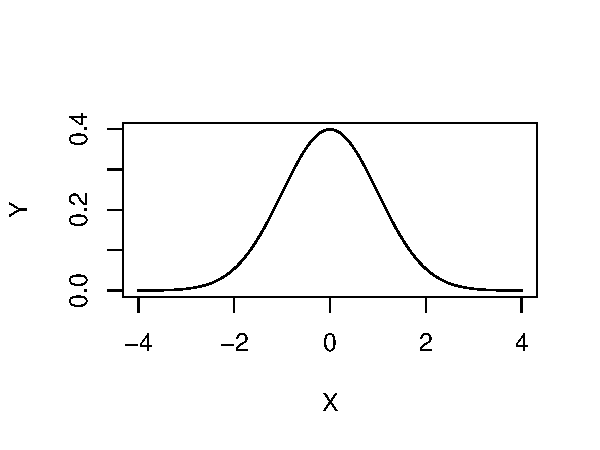
\includegraphics[width=\maxwidth]{figure/unnamed-chunk-47-1} 

}



\end{knitrout}

\subsection{Through Simulation}
The second method involves sampling randomly from the known normal distribution to simulate the probabilities that we drew directly in the above method.  In this case, we use the function \textit{rnorm}, which takes $n$ number of random samples from the normal distribution with the given mean and standard deviation.  In the \textit{hist} command, we include the specification that \textit{freq = FALSE} to make the plot reflect percentages rather than frequency counts.  
\begin{knitrout}
\definecolor{shadecolor}{rgb}{0.969, 0.969, 0.969}\color{fgcolor}\begin{kframe}
\begin{alltt}
\hlkwd{set.seed}\hlstd{(}\hlnum{1}\hlstd{)}
\hlstd{x} \hlkwb{<-} \hlkwd{rnorm}\hlstd{(}\hlkwc{n} \hlstd{=} \hlnum{100000}\hlstd{,} \hlkwc{mean} \hlstd{=} \hlnum{0}\hlstd{,} \hlkwc{sd} \hlstd{=} \hlnum{1}\hlstd{)}
\hlkwd{hist}\hlstd{(x,} \hlkwc{breaks} \hlstd{=} \hlnum{100}\hlstd{,} \hlkwc{freq} \hlstd{=} \hlnum{FALSE}\hlstd{)}
\end{alltt}
\end{kframe}

{\centering 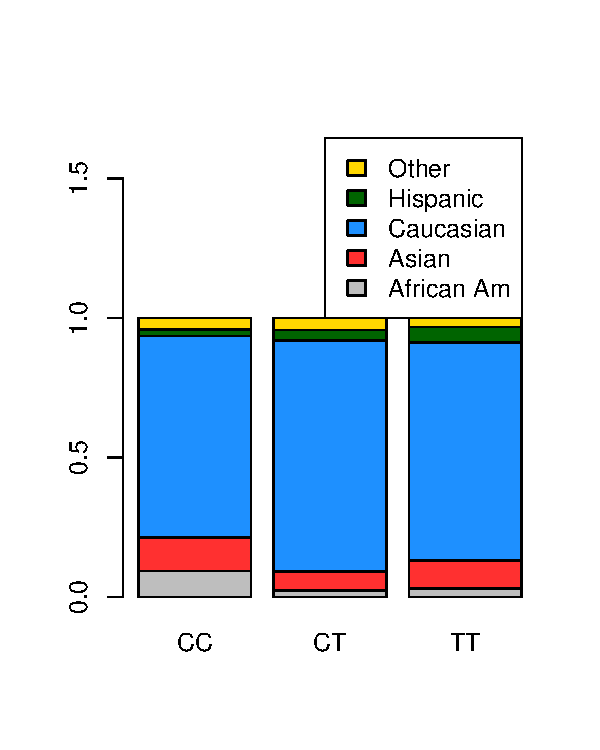
\includegraphics[width=\maxwidth]{figure/unnamed-chunk-48-1} 

}



\end{knitrout}

\subsection{A Comparison} 
To see how comparable the two methods are, we can plot them on the same graph as follows.  
\begin{knitrout}
\definecolor{shadecolor}{rgb}{0.969, 0.969, 0.969}\color{fgcolor}\begin{kframe}
\begin{alltt}
\hlkwd{hist}\hlstd{(x,} \hlkwc{freq} \hlstd{=} \hlnum{FALSE}\hlstd{,} \hlkwc{breaks} \hlstd{=} \hlnum{100}\hlstd{)}
\hlkwd{lines}\hlstd{(X,Y,} \hlkwc{col} \hlstd{=} \hlstr{"red"}\hlstd{)}
\end{alltt}
\end{kframe}

{\centering 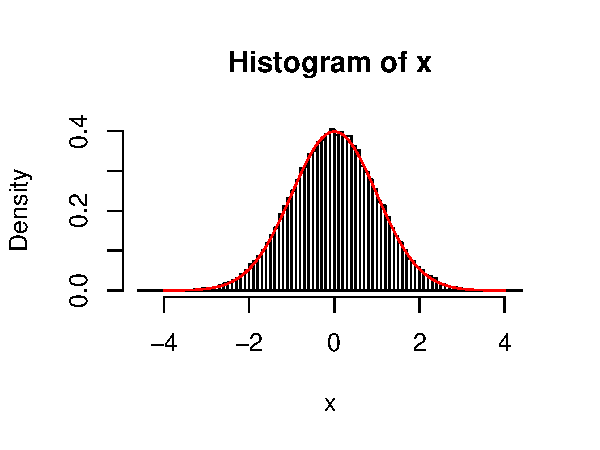
\includegraphics[width=\maxwidth]{figure/unnamed-chunk-49-1} 

}



\end{knitrout}
Note that the two show very similar results.  For practical purposes, we typically use \textit{dnorm} as it only requires one command and is the asymptotic result of simulations, rather than an approximation.  

\subsection{Probability Functions}
For the normal distribution, there are two more functions that are very useful, \textit{pnorm} and \textit{qnorm}. 

\subsubsection{pnorm} 
The function \textit{pnorm} tells you the percentage of the normal distribution that is less than or equal to the value you put in.  This corresponds to the gray area in the below plot and can be written as $pnorm(x, mean = \mu, sd = \sigma)$ which is equivalent to $P(X < x)$ where $X \sim N(\mu, \sigma)$ and $x$ is the point of interest.    
 
\begin{knitrout}
\definecolor{shadecolor}{rgb}{0.969, 0.969, 0.969}\color{fgcolor}

{\centering 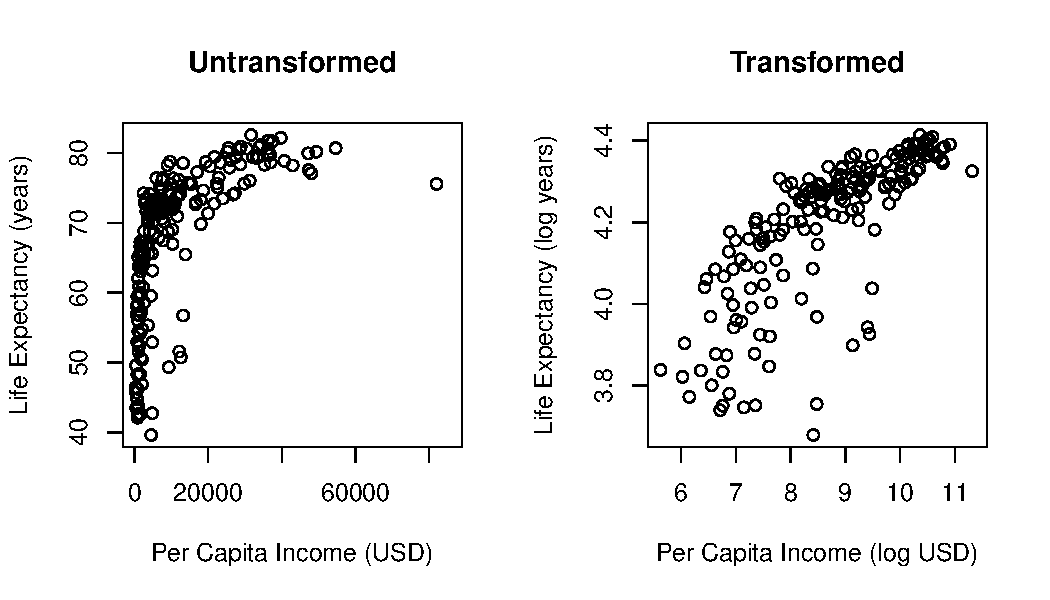
\includegraphics[width=\maxwidth]{figure/unnamed-chunk-50-1} 

}



\end{knitrout}

For some example scenarios, where we want to find a proportion of the normal distribution given $x$ or $z$, we can use the following configurations of \textit{pnorm()}: 
\begin{itemize}
\item $pnorm(z) = P(Z \leq z)$ 
\item $pnorm(z, lower.tail = FALSE) = P(Z > z)$ 
\item $pnorm(x, \mu, \sigma) = P(X \leq x)$ where $X = \sigma Z + \mu$ 
\item $pnorm(x, \mu, \sigma, lower.tail = FALSE) = P(X > x)$ where $X = \sigma Z + \mu$ 
\end{itemize}

\subsubsection{qnorm} 
On the other hand, the \textit{qnorm} function is the inverse function, instead giving the $X$ value such that the given percentage of the distribution is less than or equal to that value. This function takes a known probability and returns a value on the normal distribution that is corresponding.  

Some sample configurations of using \textit{qnorm()} can be as follows,  
\begin{itemize}
\item $qnorm(p) = P(Z \leq z)$ 
\item $qnorm(p, lower.tail = FALSE) = P(Z > z)$ 
\item $qnorm(p, \mu, \sigma) = P(X \leq x)$ where $X = \sigma Z + \mu$ 
\item $qnorm(p, \mu, \sigma, lower.tail = FALSE) = P(X > x)$ where $X = \sigma Z + \mu$ 
\end{itemize}

\section{Binomial Distribution}
The functions we saw above for the normal distribution can be similarly used for the \textbf{binomial distribution} as follows where the necessary arguments are \textit{size} and \textit{prob}
\begin{itemize} 
\item \textit{dbinom}
\item \textit{rbinom}
\item \textit{pbinom}
\item \textit{qbinom}
\end{itemize}

Similar to the above example with the normal distribution, we can use these functions in multiple ways to work with the binomial distribution.  

\subsection{Accessing the Binomial Distribution}
As we did above, we can directly access the binomial distribution using the \textit{dbinom} function as follows: 
\begin{knitrout}
\definecolor{shadecolor}{rgb}{0.969, 0.969, 0.969}\color{fgcolor}\begin{kframe}
\begin{alltt}
\hlcom{## Splitting the graphics window into two panes }
\hlkwd{par}\hlstd{(}\hlkwc{mfrow}\hlstd{=}\hlkwd{c}\hlstd{(}\hlnum{1}\hlstd{,}\hlnum{2}\hlstd{))}
\hlcom{## Directly plotting the binomial distribution}
 \hlcom{# getting a list of values to evaluate distribution}
\hlstd{X} \hlkwb{=} \hlkwd{seq}\hlstd{(}\hlnum{0}\hlstd{,} \hlnum{10}\hlstd{,} \hlnum{1}\hlstd{)}
 \hlcom{# getting normal distribution value of the given X values }
\hlstd{Y} \hlkwb{=} \hlkwd{dbinom}\hlstd{(X,} \hlkwc{size} \hlstd{=} \hlnum{10}\hlstd{,} \hlkwc{prob} \hlstd{=} \hlnum{.25}\hlstd{)}
 \hlcom{# plotting results }
\hlkwd{plot}\hlstd{(X,Y,} \hlkwc{type} \hlstd{=} \hlstr{"s"}\hlstd{,} \hlkwc{main} \hlstd{=} \hlstr{"Direct Plot"}\hlstd{,} \hlkwc{xlim} \hlstd{=} \hlkwd{c}\hlstd{(}\hlnum{0}\hlstd{,}\hlnum{10}\hlstd{))}

\hlcom{## Instead Using Simulation}
\hlkwd{set.seed}\hlstd{(}\hlnum{1}\hlstd{)}
\hlstd{x} \hlkwb{<-} \hlkwd{rbinom}\hlstd{(}\hlkwc{n} \hlstd{=} \hlnum{100000}\hlstd{,} \hlkwc{size} \hlstd{=} \hlnum{10}\hlstd{,} \hlkwc{prob} \hlstd{=} \hlnum{.25}\hlstd{)}
\hlkwd{hist}\hlstd{(x,} \hlkwc{breaks} \hlstd{=} \hlnum{10}\hlstd{,} \hlkwc{freq} \hlstd{=} \hlnum{FALSE}\hlstd{,}\hlkwc{right} \hlstd{=} \hlnum{FALSE}\hlstd{,} \hlkwc{main} \hlstd{=} \hlstr{"Simulation"}\hlstd{,} \hlkwc{xlim} \hlstd{=} \hlkwd{c}\hlstd{(}\hlnum{0}\hlstd{,}\hlnum{10}\hlstd{))}
\hlkwd{box}\hlstd{()}
\end{alltt}
\end{kframe}

{\centering 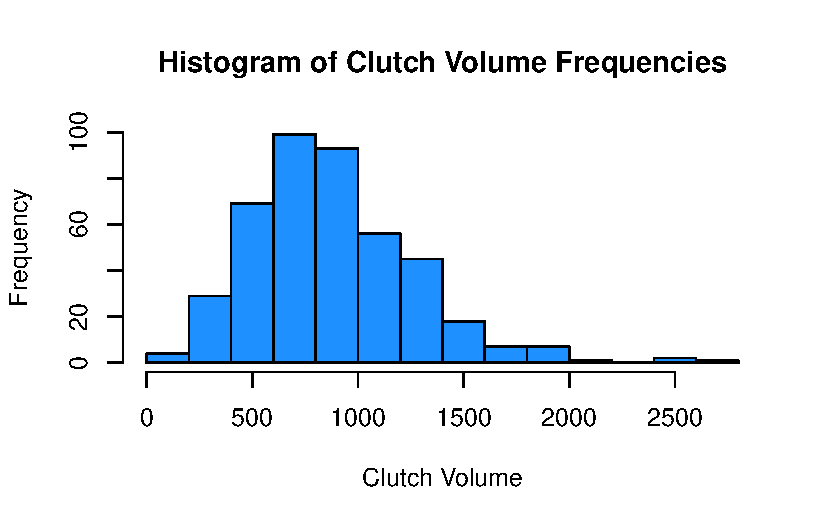
\includegraphics[width=\maxwidth]{figure/unnamed-chunk-51-1} 

}



\end{knitrout}

\subsection{Comparison of the Methods}
\begin{knitrout}
\definecolor{shadecolor}{rgb}{0.969, 0.969, 0.969}\color{fgcolor}\begin{kframe}
\begin{alltt}
\hlkwd{hist}\hlstd{(x,} \hlkwc{breaks} \hlstd{=} \hlnum{10}\hlstd{,} \hlkwc{freq} \hlstd{=} \hlnum{FALSE}\hlstd{,}\hlkwc{right} \hlstd{=} \hlnum{FALSE}\hlstd{)}
\hlkwd{lines}\hlstd{(X,Y,} \hlkwc{type} \hlstd{=} \hlstr{"s"}\hlstd{,} \hlkwc{col} \hlstd{=} \hlstr{"red"}\hlstd{)}
\end{alltt}
\end{kframe}

{\centering 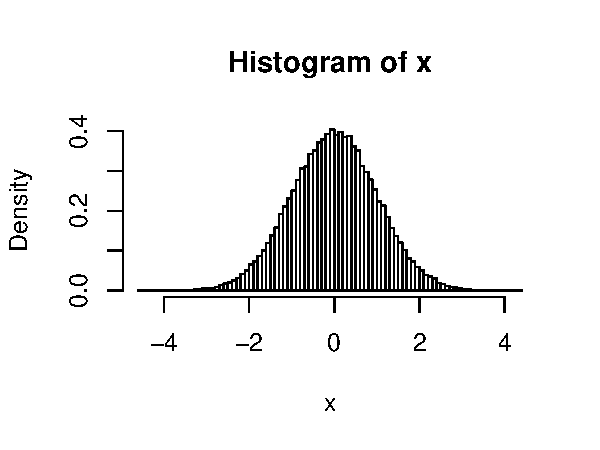
\includegraphics[width=\maxwidth]{figure/unnamed-chunk-52-1} 

}



\end{knitrout}

\section{Continuous and Discrete Distributions}


\section{Poisson Distribution}
Similarly, we can build out the functions for the \textbf{poisson distribution} as the following where the necessary argument is \textit{lambda}
\begin{itemize} 
\item \textit{dbinom}
\item \textit{rbinom}
\item \textit{pbinom}
\item \textit{qbinom}
\end{itemize}

\section{Geometric Distribution}
We can follow the same pattern for the \textbf{geometric distribution} to get the following where the necessary argument is \textit{prob}
\begin{itemize} 
\item \textit{dgeom}
\item \textit{rgeom}
\item \textit{pgeom}
\item \textit{qgeom}
\end{itemize}

\section{Negative Binomial Distribution}
Finally, we can follow the same pattern for the \textbf{negative binomial distribution} to get the following where the necessary arguments are \textit{prob} and \textit{size}
\begin{itemize} 
\item \textit{dnbinom}
\item \textit{rnbinom}
\item \textit{pnbinom}
\item \textit{qnbinom}
\end{itemize}



\newpage 
\chapter{Chapter 4 - Name this}
\minitoc

\vspace{0.5cm} 


\end{document}
